 %----------------------------------------------------------------------------------------
%	PREÁMBULO
%----------------------------------------------------------------------------------------

% !TeX TXS-program:compile = txs:///pdflatex/[--shell-escape]
\documentclass[11pt, oneside]{book}
\usepackage[paperwidth=17cm, paperheight=22.5cm, bottom=2.5cm, right=2.5cm]{geometry}

% El borde inferior puede parecerles muy amplio a la vista. Les recomiendo hacer una prueba de impresión antes para ajustarlo

\usepackage{amssymb,amsmath,amsthm} % Símbolos matemáticos
\usepackage[spanish,mexico,es-tabla]{babel}
\usepackage[utf8]{inputenc} % Acentos y otros símbolos 
\usepackage{enumerate}
\usepackage{optidef}
\usepackage{hyperref} % Hipervínculos en el índice
\usepackage[spanish]{cleveref}
\usepackage{graphicx}
\usepackage[usenames,dvipsnames]{xcolor} % Color
%\usepackage{subfig} % Subfiguras
\usepackage{listings}%Para los códigos de MALTAB, ver documentación de matlab-prettifier
\usepackage[framed]{matlab-prettifier}
\usepackage[linesnumbered,lined,boxruled,spanish,onelanguage]{algorithm2e}
\usepackage{titling}
\usepackage{amsfonts}
\usepackage[thinc]{esdiff}
\spanishdecimal{.}
\definecolor{itamgreen}{RGB}{0,104,83}
\hypersetup{
    colorlinks=true,
    linkcolor=itamgreen,
    filecolor=itamgreen,      
    urlcolor=itamgreen,
    citecolor=itamgreen
}
\urlstyle{same}


\usepackage{translations}
\graphicspath{{Imagenes/}} % En qué carpeta están las imágenes

\DeclareTranslationFallback{rank}{rank}
\DeclareTranslation{english}{rank}{rank}
\DeclareTranslation{spanish}{rank}{rango}

\DeclareMathOperator{\rank}{\GetTranslation{rank}}


% Para eliminar guiones y justificar texto
\tolerance=1
\emergencystretch=\maxdimen
\hyphenpenalty=10000
\hbadness=10000

\linespread{1.25} % Asemeja el interlineado 1.5 de Word

\let\oldfootnote\footnote % Deja espacio entre el número del pie de página y el inicio del texto
\renewcommand\footnote[1]{%
\oldfootnote{\hspace{0.05mm}#1}}

\newcommand{\bigO}[1]{\ensuremath{\mathop{}\mathopen{}\mathcal{O}\mathopen{}\left(#1\right)}}

\newcommand\smallO[1]{
    \mathchoice
    {% mode \displaystyle
      \scriptstyle\mathcal{O}\left(#1\right)
    }
    {% mode \textstyle
      \scriptstyle\mathcal{O}\left(#1\right)
    }
    {% mode \scriptstyle
      \scriptscriptstyle\mathcal{O}\left(#1\right)
    }
    {% mode \scriptscriptstyle
      \scalebox{0.7}{$\scriptscriptstyle\mathcal{O}$}\left(#1\right)
    }
}
  

\renewcommand{\thefootnote} {\textcolor{Black}{\arabic{footnote}}} % Súperindice a color negro

\setlength{\footnotesep}{0.75\baselineskip} % Espaciado entre notas al pie

\usepackage{fnpos} % Footnotes al final de pág.

\usepackage[justification=centering, font=bf, labelsep=period, skip=5pt]{caption} % Centrar captions de tablas y ponerlas en negritas

\newcommand{\imagesource}[1]{{\footnotesize Fuente: #1}}

\usepackage{tabularx} % Big tables
\usepackage{adjustbox}
\usepackage{longtable}


\usepackage{float} % Float tables

\usepackage{pgfplots} % Gráficas
\pgfplotsset{compat=newest}
\pgfplotsset{width=7.5cm}
\pgfkeys{/pgf/number format/1000 sep={}}

\newtheorem{theorem}{Teorema}[chapter]
\newtheorem{corollary}{Corolario}[theorem]
\newtheorem{lemma}[theorem]{Lema}
\newtheorem{definition}{Definición}
\newtheorem{plain}{Proposición}
\newtheorem{remark}{Corolario}[plain]

\newcommand{\Tr}[1]{\operatorname{Tr}\left(#1\right)}
\newcommand{\diag}[1]{\operatorname{diag}\left(#1\right)}
\newcommand{\frNm}[1]{\left\|#1\right\|_{\mathrm{F}}}

\SetKwBlock{Loop}{Repetir}{fin}

\usepackage{afterpage}
\newcommand\myemptypage{
    \null
    \thispagestyle{empty}
    \newpage
    }
    
    
\usepackage{todonotes}
%HAY Q BORRAR ESTOS COMMANDS EVENTUALMENTE
\newcommand{\val}[1]{\todo[color=blue!20!white]{\textbf{Vale:} #1}}
\newcommand{\valinline}[1]{\todo[inline,color=blue!20!white]{\textbf{Vale:} #1}}

\usepackage{natbib}

\usepackage{tcolorbox}

\usepackage{dirtytalk}

\usepackage[cache=false]{minted}
\usemintedstyle{bw}

\usepackage{multirow}

\begin{document}

%----------------------------------------------------------------------------------------
%	PORTADA
%----------------------------------------------------------------------------------------



\title{Una tesis extendida ($\overline{\text{tesis}}$)} 
\author{Valeria Aurora Pérez Chávez}

\begin{titlepage}
\begin{center}

\textsc{\Large Instituto Tecnológico Autónomo de México}\\[2em]

%Figura
\begin{figure}[h]
\begin{center}

\includegraphics[scale=0.9]{logo-ITAM.pdf}
\end{center}
\end{figure}

% Pueden modificar el tamaño del logo cambiando la escala

\textbf{\LARGE \thetitle}\\[2em]

\textsc{\large Tesis}\\[1em]

\textsc{\large que para obtener el título de}\\[1em]

\textsc{\LARGE Licenciado en Matemáticas Aplicadas}\\[1em]

\textsc{\large Presenta}\\[1em]

\textsc{\LARGE \theauthor}\\[1em]

\textsc{\large Asesor: Ernesto Juvenal Barrios Zamudio}\\[1em]


% Asegúrense de escribir el nombre completo de su asesor con grado académico

\end{center}

\vspace*{\fill}
\textsc{Ciudad de México \hspace*{\fill} 2021} %El otro año es el bueno

\end{titlepage}



%----------------------------------------------------------------------------------------
%	DECLARACIÓN
%----------------------------------------------------------------------------------------

\thispagestyle{empty}

\vspace*{\fill}
\begingroup

\noindent
«Con fundamento en los artículos 21 y 27 de la Ley Federal del Derecho de Autor y como titular de los derechos moral y patrimonial de la obra titulada ``\textbf{\thetitle}'', otorgo de manera gratuita y permanente al Instituto Tecnológico Autónomo de México y a la Biblioteca Raúl Bailléres Jr., la autorización para que fijen la obra en cualquier medio, incluido el electrónico, y la divulguen entre sus usuarios, profesores, estudiantes o terceras personas, sin que pueda percibir por tal divulgación una contraprestación.»


\centering 

\vspace{3em}

\textsc{\theauthor}

\vspace{5em}

\rule[1em]{20em}{0.5pt} % Línea para la fecha

\textsc{Fecha}
 
\vspace{8em}

\rule[1em]{20em}{0.5pt} % Línea para la firma

\textsc{Firma}

\endgroup
\vspace*{\fill}

\newpage


%----------------------------------------------------------------------------------------
%	DEDICATORIA
%----------------------------------------------------------------------------------------

\thispagestyle{empty}
\pagenumbering{gobble}

\chapter*{Agradecimientos}

Agradezco a facu por ser tan chingona y a Mike por pasarme el formato. Salu2.
\begin{flushright}
\textsc{El Serch}
\end{flushright}
\newpage


\pagestyle{plain}
\frontmatter
%----------------------------------------------------------------------------------------
%	RESUMEN
%----------------------------------------------------------------------------------------
\include{Chapters/Resumen}


%----------------------------------------------------------------------------------------
%	ÍNDICE GENERAL
%---------------------------------------------------------------------------------------

\tableofcontents %Opcional pero sugerido, en especial si como Paco van a escribir un libro de 500 páginas. Es tesis, no enciclopedia.

%----------------------------------------------------------------------------------------
%	ÍNDICE DE CUADROS Y FIGURAS
%---------------------------------------------------------------------------------------

\listofalgorithms %Opcional
\newpage

\listoftables %Opcional

\listoffigures %Opcional

%----------------------------------------------------------------------------------------
%	TESIS
%----------------------------------------------------------------------------------------

\mainmatter % Empieza la numeración de las páginas

\pagestyle{plain}

% Incluye los capítulos en el fólder de capítulos

\chapter{Introducción}

\say{I always promote \textsf{Julia} among friends and colleagues in Latin America, even when it has been difficult to convince them because of the scarce resources of \textsf{Julia} in Spanish. I firmly believe in open access knowledge without barriers (either language barriers, accessibility, or others), and I will always advocate for that} \cite{articulo_10anos}. Las palabras de la chilena Pamela Bustamente, usuaria de \textsf{Julia},  engloban la razón de ser de esta tesis. 

Mi camino con \textsf{Julia} comenzó a principios del 2021 cuando tuve la oportunidad de trabajar en el Instituto Mexicano del Seguro Social (IMSS). \textsf{Julia} fue la herramienta que utilice para desarrollar un proyecto que estaba fundamentado en estadística bayesiana y requería de una gran cantidad de simulaciones. No tarde mucho tiempo en encontrarme con las dificultades que menciona Pamela y algunas más. Sin embargo, \textsf{Julia} debe tener otras cualidades que frecuentemente lo destaquen como un lenguaje prometedor que cada día va tomando más fuerza en la comunidad de programadores. 

Al principio, dichas cualidades eran un misterio para mí. Mi interrogante principal fue sobre la necesidad de crear este nuevo lenguaje. ¿Por qué usar \textsf{Julia} y no \textsf{Python} o \textsf{R}?, ¿Cuál fue la motivación de su creación? y, después de encontrarme con una falta de recursos, ¿Cómo es posible que 10 años más tarde hay tan poca ayuda de este lenguaje?  Esta tesis es mi esfuerzo por mostrar un nuevo lenguaje, sus alcances y hacer una comparativa con lo que ya se conoce. De paso, mi trabajo queda como evidencia y punto de partida para futuros usuarios hispanohablantes.  

Este trabajo no es un manual de \textsf{Julia} ni de ningún otro lenguaje. Eso ya existe. Lo que se busca es explicar pros y contras que se encontraron al utilizar \textsf{Julia}, \textsf{Python} y \textsf{R} en tres ejercicios distintos.

La tesis se divide en dos partes. El propósito de la primera parte es dar una imagen general de las funciones que se utilizaron en los tres lenguajes para crear la segunda parte. Primero, se expone la instalación de \textsf{Julia} en un sistema operativo \textsf{Windows} para después explicar aspectos básicos del lenguaje. También, se da una introducción a dos paquetes fundamentales para este trabajo. Esto se hace pensando que \textsf{Julia} es el lenguaje más reciente y se busca que el lector navegue fácilmente por el código presentado. Después, se presentan los paquetes y funciones que se utilizaron en \textsf{Python} y en \textsf{R} suponiendo que el lector ya está familiarizado con ellos. 

La segunda parte de la tesis consta de tres ejercicios cuyo objetivo es mostrar un aspecto diferente en los lenguajes. El primer ejercicio toma datos del National Institute of Standards and Technology (NIST) para medir la precisión numérica de cada lenguaje al hacer el ajuste de un polinomio de grado 10. El segundo ejercicio usa los datos del Censo de Población y Vivienda de México del 2020 hecho por el Instituto Nacional de Estadística y Geografía (INEGI). El objetivo de este ejercicio es el manejo y manipulación de una gran cantidad de datos. Finalmente, el tercer ejercicio presenta la programación de un algoritmo de búsqueda que se utiliza en la discriminación de modelos en diseños de experimentos. En este ejercicio, los cálculos son más intensivos por lo que busca medir la capacidad y velocidad de cómputo de los lenguajes. 

A continuación, se comienza este trabajo con la presentación de \textsf{Julia}. 




\chapter{Julia}

Julia es un lenguaje de programación gratis cuyo propósito general es ser tan rápido como C, pero manteniendo la facilidad de lenguaje de R o Python. Es una combinación de sintaxis simple con alto rendimiento computacional. Su slogan es "Julia se ve como Python, se siente como Lisp, corre como Fortran" \citep{Hackers}. 
Esta combinación de características hace que Julia sea un lenguaje de programación que ha tomado mucha fuerza en la comunidad científica. Ya que no es un lenguaje muy conocido, en esta sección explicaré como instalar Julia en una computadora con sistema Windows y algunos de los básicos del lenguaje.

\section{Reproducibilidad}
Antes de empezar, es necesario enfatizar que esta tesis es completamente reproducible. En Peng y Hicks definen que \say{un análisis de datos publicado es reproducible si el conjunto de datos y el código utilizados para crear el análisis de datos está disponible para que otros lo analicen y estudien de manera independiente} \cite{peng2021reproducible}. A pesar de que en el artículo enfatizan que esta definición puede ser un poco ambigua, sí resaltan que la reproducibilidad es un medio para revisar y, posteriomente, confiar en el análisis de otros. 

Por lo tanto, para este trabajo decidí publicar el código que utilicé en \textsf{GitHub}. Además, hago hincapié en las fuentes de los datos. A pesar de que esta tesis no es un manual de Julia, Python o R considero da suma importancia publicar mi trabajo para que les sirva a mis compañeros como referencia o punto de partida. 


\section{Instalación}
Este trabajo está hecho y escrito en Windows, por lo que explicaré la instalación de Julia y todas las demás aplicaciones en este sistema operativo. Sin embargo, sé que la instalación en Mac y Linux es muy similar y usualmente las instrucciones a seguir vienen en las mismas páginas que Windows. 

Al momento de la escritura y publicación de esta tesis la versión de Julia disponible es la \textbf{v1.6.3}. El primer paso ara descargar Julia, es entrar al link \url{https://julialang.org/downloads/}. 


En esta versión de Julia, las opciones disponibles de descarga son un instalador de 64-bits o uno de 32-bits. Para saber el tipo de Sistema que tiene tu ordenador debes seleccionar el botón de \textsf{Start}, después \textsf{Configuración} $>$ \textsf{Sistema} $>$ \textsf{Acerca de}. En esta opción puedes ver el tipo de sistema que tiene tu computadora. Con esta información, puedes elegir el instalador para tu computadora. Es importante seleccionar el \textsf{installer} y no el \textsf{portable}. Una vez descargado, seleccionas el archivo \textsf{.exe} y sigues los pasos de instalación. 

\section{Símbolo del sistema}
Una vez instalado puedes correr Julia desde el símbolo de sistema o desde otro programa como Atom, Visual Studio Code o Jupyter Notebook. Una de las ventajas de utilizar Julia desde el símbolo de sistema (también conocido como \textit{Command Prompt} o cmd) es que puedes controlar algunos parámetros del lenguaje. Mi sugerencia es que comiences a usar Julia directo desde el ícono que se genera automáticamente en la descarga. Después, cuando entiendas lo básico y empieces a generar programas que requieran mayor nivel computacional comiences a utilizar el cmd para correr Julia. Para facilitar esto, te recomiendo agregar Julia a un \textbf{PATH}. Las instrucciones para hacerlo en Windows 10 están en la página \url{https://julialang.org/downloads/platform/#windows}.

\subsection{\textit{Multithreading}}
Una de las razones por la que Julia tiene más velocidad que otros lenguajes es porque  tiene la capacidad para multihilo (\textit{multithreading} en inglés). Esto significa que puede correr diferentes tareas de manera simultánea en varios hilos. Explicado de la manera más simple, la meta de los autores de Julia fue hacer un lenguaje de programación con un rendimiento tan alto que pudiera hacer varias cosas a la vez. Debido a que uno de los objetivos de esta tesis es medir la eficiencia y velocidad de Julia, es crucial conocer la característica del \textit{multithreading} y como utilizarla. 

Si estás usando Julia por medio del cmd es necesario modificar la cantidad de hilos que se van a utilizar antes de ejecutar Julia.  En Windows, esto se hace escribiendo \texttt{set JULIA\_ NUM\_ THREADS=4} \citep{manual_Julia}. Si estás trabajando con otro sistema operativo, este link te puede ayudar a cambiar la cantidad de hilos \url{https://docs.julialang.org/en/v1/manual/multi-threading/}. En este ejemplo, se cambiaron los hilos a 4, pero se puede poner cualquier número. Sin embargo, se recomienda que el número no exceda de la cantidad de procesadores físicos de la computadora. Después de hacer esta modificación, ahora sí podemos ejecutar Julia. 
  
Para observar que el cambio se ejecutó de manera correcta (en cualquiera de las dos opciones) basta con correr el comando \texttt{Threads.nthreads()} y observar que la respuesta sea el número deseado. 

\section{Básicos de Julia}
Como ya se mencionó, Julia busca ser un lenguaje de programación sencillo e intuitivo. Por lo tanto, su sintaxis es bastante sencilla. La asignación de variables se hace con un signo de igualdad $=$. El ejemplo más sencillo de esto sería \texttt{x = 2} donde denotamos a x el valor de 2. Toda la información sobre la sintaxis que utiliza Julia la obtuve del manual oficial de Julia \citep{manual_Julia}.

\subsection{Operaciones básicas}
La tabla \ref{operaciones_basicas_Julia} muestra la sintaxis usada para las operaciones básicas en Julia. 


\begin{center}
	\begin{tabular}{|c|c|c|} 
		\hline
		Expresión & Nombre & Descripción \\ 
		\hline 
		\texttt{+x} & suma unaria & la operación identidad \\ 

		\texttt{-x} & resta unaria & asigna a los valores sus inversos aditivos \\ 

		\texttt{x + y} & suma binaria & realiza adición \\ 

		\texttt{x - y} & resta binaria & realiza sustracción \\

		\texttt{x * y} & multiplicación & realiza multiplicación \\

		\texttt{x / y} & división & realiza divisiones \\

		\texttt{x $\div$ y} & división de enteros & $x / y$ truncado a un entero \\

		\texttt{x $\setminus$ y} & división inversa & equivalente a dividir \texttt{y / x} \\

		\texttt{x $\wedge$ y} & potencia & eleva \texttt{x} a la potencia \texttt{y} \\

		\texttt{x \% y} & residuo & equivalente a \texttt{rem(x,y)} \\
		
		\texttt{!x} & negación & realiza lo contrario de \texttt{x} \\
		
		\texttt{x \& \& y} & \textit{and} lógico & verifica si \texttt{x} y \texttt{y} se cumplen \\
		
		\texttt{x || y} & \textit{or} lógico & verifica si al menos uno, \texttt{x} o \texttt{y},  se cumplen \\
		\hline
	\end{tabular} 
	\captionof{table}{Operaciones básicas en Julia} \label{operaciones_basicas_Julia}
\end{center}


\subsubsection{Operaciones básicas en vectores}
En Julia, para cada operación binaria existe su correspondiente operación punto (\textit{dot operation} en inglés). Estas funciones están definidas para efectuarse elemento por elemento en vectores y matrices. Para llamarse, basta agregar un punto antes del operador binario. Por ejemplo,
 \texttt{[1 9 9 7] .$\wedge$ 2} eleva cada uno de los elementos del vector al cuadrado. 

También es importante mencionar que Julia maneja los números imaginarios utilizando el sufijo \texttt{im}. Sin embargo, no los utilice en este trabajo omitiré dar una mayor explicación. 

\subsection{\textit{Strings} (secuencias de caracteres)} 

Además de números, Julia puede asignar characteres a variables. Esto se hace utilizando las comillas dobles. Similar a otros lenguajes de programación, podemos accesar a caracteres específicos de un string utilizando corchetes cuadrados $[$ $]$ y a cadenas seguidas de caracteres usando dos puntos $:$. Por ejemplo,

\begin{minted}{julia}
    julia> string = "Esta tesis es genial"
    julia> string[6]
    't': ASCII/Unicode U+0074 (category Ll: Letter, lowercase)
    
    julia> string[4:8]
    "a tes"
\end{minted}


Además, Julia también cuenta con la opción de concatenación de múltiples strings. Esto se hace utilizando un asterisco $*$ para separar cada uno de los strings. Por ejemplo,

\begin{minted}{julia}
	julia> grado = "licenciada"
	julia> nexo = "en"
	julia> carrera = "matematicas aplicadas"
	julia> espacio = " "
	julia> grado*espacio*nexo*espacio*carrera
	"licencia en matematicas aplicadas"
\end{minted}

\subsection{Funciones}
En Julia, una función es un objeto que asigna una tupla de argumentos a un valor de retorno \citep{Julia_manual}. La sintáxis básica para definir funciones en Julia es 

\begin{minted}{julia}
	function f(x, y)
		x + y
	end
\end{minted}

Además, puedes agregar la palabra \textit{return} para que la función regrese un valor. Por ejemplo, si quisieramos tener una función a la que le des dos números y te regrese el número mayor, la función sería la siguiente:

\begin{minted}{julia}
	function numero_mayor(x, y)
		if (x > y)
			return x
		else
			return y
		end
	end
\end{minted}


Para llamar a la función bastaría con escribir \texttt{numero\_mayor(x, y)} asignando o sustituyendo valores por $x$ y $y$. 

\subsection{Vectores y Matrices}

\begin{definition}
Un vector columna de $n$ componentes se define como un conjunto ordenado de $n$ números escritos de la siguiente manera:
\begin{equation*}
    \begin{aligned}
    \begin{pmatrix}
    x_1 \\ 
    x_2 \\
    \vdots \\
    x_n
    \end{pmatrix} 
    \end{aligned}
\end{equation*}
\end{definition}


En Julia, para definir un vector columna se hace uso de los corchetes cuadrados $[$ $]$ y comas. Por ejemplo, 

\begin{minted}{julia}
	julia> A = [1, 9, 9, 7]
	4-element Vector{Int64}
	1
	9
	9
	7
\end{minted}

da como resultado un vector de 4 elementos de tipo Int64. Es muy importante aprender a identificar como Julia lee los objetos ya que cada objeto tiene características y funciones diferentes.  

Si quisiera definir un vector renglón, se hace exactamente igual solamente omitiendo el uso de las comas. Sin embargo, es importante señalar que  ahora Julia tomó el objeto A como una matriz, no como un vector. 

\begin{definition}
Una matriz $A$ de $m \times n$ es un arreglo rectangular de $mn$ números dispuestos en $m$ renglones y $n$ columnas. 

\begin{equation*}
    \begin{aligned}
    \begin{pmatrix}
    a_{11} & a_{12} & \dots & a_{1j} & \dots & a_{1n} \\
    a_{21} & a_{22} & \dots & a_{2j} & \dots & a_{2n} \\
    \vdots &  \vdots  &  \ddots &  \vdots  & \ddots &\vdots\\
    a_{i1} & a_{i2} & \dots & a_{ij} & \dots & a_{in} \\
    \vdots &  \vdots  &  \ddots &  \vdots  & \ddots &\vdots\\
     a_{m1} & a_{m2} & \dots & a_{mj} & \dots & a_{mn} \\
    \end{pmatrix} 
    \end{aligned}
\end{equation*}
\end{definition}


En Julia, hay dos formas de definir matrices. La primera es utilizando los corchetes cuadrados $[$ $]$ para comenzar y terminar la matriz. Las columnas están separadas por espacios y las filas por punto y coma. La segunda opción similar a la primera con la única diferencia de que en lugar de punto y coma se cambia de renglón. Esta opción puede ser un poco tediosa ya que requieren que las columnas estén alineadas. Sin embargo, es una forma más visual de ver las matrices. En la siguiente tabla se pueden ver ambas opciones. 

\begin{minted}{julia}
	julia> A_1 = [1 2 3; 4 5 6]
	2x3 Matrix{Int64}
	1 2 3
	4 5 6
	julia> A_2 = [1 2 3
				4 5 6]
	2x3 Matrix{Int64}
	1 2 3
	4 5 6

\end{minted}

De manera análoga con los vectores, para llamar un solo elemento de la matriz se utilizan los corchetes cuadrados. Continuando con el ejemplo anterior, para obtener el número 5 de la matriz $\text{A\_2}$, se programaría el código $\texttt{A\_2[2, 2]}$.

Es importante mencionar que como muchos otros lenguajes, Julia ya tiene programadas las operaciones básicas de las matrices en el paquete \textsf{Linear Algebra}. El catálogo de funciones es bastante extenso para incluirlo en este trabajo, pero lo puedes encontrar en \url{https://docs.julialang.org/en/v1/stdlib/LinearAlgebra/}.

\subsection{Instalación de un paquete}
Para hacer cualquier otra operación fuera de lo básico que ya mencioné, Julia hace uso de paquetes. Los paquetes son similar a las librerías en R. La lista completa de paquetes registrados en Julia se encuentra en \url{https://juliapackages.com/}. 

Lo primero que hay que saber sobre estos paquetes es como descargarlos y agregarlos. Antes de buscar instalar cualquier paquete primero hay que usar el paquete \textbf{Pkg} que ya viene por default cuando descargas Julia. Después, hay que usar el comando \textbf{Pkg.add} para agregar el paquete nuevo. Finalmente, llamas al paquete con el comando \textbf{using}. A continuación está un resumen de lo anterior. 

\begin{minted}{julia}
	using Pkg
	Pkg.add("paquete_nuevo")
	using paquete_nuevo
\end{minted}

Después, cada vez que vayas a utilizar un paquete basta con llamar al paquete con el comando \textbf{using}. 
En las siguientes secciones explico y ejemplifico el uso de dos paquetes muy usados en esta tesis. 

\subsection{\textit{DataFrames}}

Un \textit{dataframe} es una tabla estructurada de dos dimensiones que se usa para tabular distintos tipos de datos. Julia tiene un paquete llamado \textit{DataFrames}  que permite trabajar con dataframes de creación propia o de alguna fuente externa. 


\subsubsection{Crear un dataframe}

Aunque de manera general los dataframes se utilicen para manejar grandes cantidades de información exportada de otros formatos, es importante saber como se crea y manipula un dataframe desde cero en Julia. Hacerlo es simple. Primero, hay que escribir la palabra \texttt{DataFrame} y abrir un paréntesis. Después, se escribe el nombre de la primera columna, un signo de igualdad y los datos que corresponden a esa variable. Se repite lo mismo con la cantidad de columnas que se requieran. Por ejemplo, para hacer un dataframe con las claves únicas y nombres de cinco mujeres el código sería el siguiente: 


\begin{minted}{julia}
    df = DataFrame(id = 1:5, 
    nombre = ["Valeria", "Paula", "María José", 
        "Sofía", "Mónica"])
\end{minted}

Es importante nombrar las columnas del dataframe ya que de esta forma basta con escribir \texttt{df.col} para referirnos a la columna (en este caso llamada 'col') dataframe llamado df. De la misma manera, si se quisiera agregar una columna nueva basta con asignarle datos a \texttt{df.colNueva}. Por ejemplo, si quisieras agregar una columna llamada \texttt{color} al dataframe del ejemplo anterior, el código sería el siguiente: 

\begin{minted}{julia}
     df.color = ["morado", "azul", "verde", "negro", "rojo"]
\end{minted}

Como cualquier otro objeto en Julia, los dataframes tienen diferentes funciones. Es posible seleccionar un subgrupo de datos, agregar datos por renglones, modificar y eliminar datos, etc. Sin embargo, eso no es de relevancia para esta tesis por lo que lo omitiré.

\subsubsection{Importar datos en un dataframe}

Como ya mencioné, los dataframes son utilizados para contener grandes cantidades de información. Usualmente, esta información no es generada en Julia, por lo que hay importarla. Una de las formas más rápidas es usando el paquete \texttt{CSV}. Recuerda que para usarlo por primera vez hay que seguir los pasos descritos en \ref{instalacion_paquete}. 

Una vez instalado el programa, basta utilizar el comando \texttt{CSV.read} y la ruta de la ubicación del archivo para exportar los datos. 

\begin{minted}{julia}
     df = CSV.read("C:/Users/Valeria/Documents/ejemplo.csv", DataFrame)
\end{minted}

\valinline{Tengo que arreglar esto sí o sí}

\begin{figure}[h]
\begin{center}
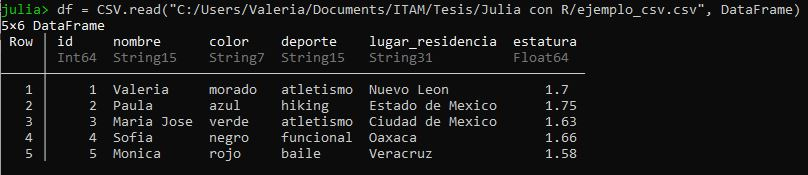
\includegraphics[scale=0.6]{Imagenes/insertar_df.JPG}
  \label{insertar_df}
\end{center}
\end{figure}

Los dataframes se pueden manejar de diferentes maneras. En este trabajo utilicé algunas de ellas, pero en caso de que tengas más dudas puedes consultar el manual oficial del paquete en \url{https://dataframes.juliadata.org/stable/}. 

\subsection{Regresiones}

\valinline{Buen link de ayuda \url{https://www.machinelearningplus.com/linear-regression-in-julia/}}

¿Cuál es el punto de tener una muestra de tamaño significativo si no sabemos analizarla? Una de las maravillas que nos regala la estadística es el uso de regresiones para intentar encontrar una explicación a los datos. Regresión es un método que permite a los investigadores resumir como predicciones o valores promedio de un resultado varían a través de variables individuales definidas como predictores. \citep{regression_other_stories} 

En pocas palabras, una regresión es una fórmula que intenta explicar como una variable depende otras. En Julia, esto se puede hacer con ayuda del paquete \texttt{GLM}, ya que facilita el cálculo de modelos lineales. Como todos los paquetes, primero hay que instalarlo usando los pasos en \ref{instalacion_paquete}. 

En este paquete la función principal se llama \texttt{glm}. En el manual oficial del paquete \cite{glm_manual} está descrita la manera en que se pueden generar modelos más avanzados. La función principal es \texttt{glm(formula, data, family, link)} donde 

\begin{itemize}
    \item \texttt{formula}: usa los nombres de las columnas del dataframe de datos para referirse a las variables predictoras
    
    \item \texttt{data}: el dataframe que contenga los predictores de las formula
    
    \item \texttt{family}: podemos elegir entre Bernoulli(), Binomial(), Gamma(), Normal(), Poisson() o NegativeBinomial() 
    
    \item \texttt{link}: se usa para especificar la función liga o \textit{link function}. La lista de posibles opciones está en el manual oficial de GLM. 
\end{itemize}


\subsubsection{Regresión lineal simple}
El modelo de regresión lineal más simple es el que tiene un solo predictor

\begin{equation*}
    \begin{aligned}
    y = a + bx + \epsilon
    \end{aligned}
\end{equation*}

Para ejemplificar este modelo de regresión use los datos de \citep{regression_other_stories}. Los datos fueron recabados por Douglas Hibbs con el objetivo de predecir las elecciones de Estados Unidos basándose solamente en el crecimiento económico. Los datos se ven de la siguiente manera: \val{Como le hago para incluir esto?}

\begin{figure}[H]
\begin{center}
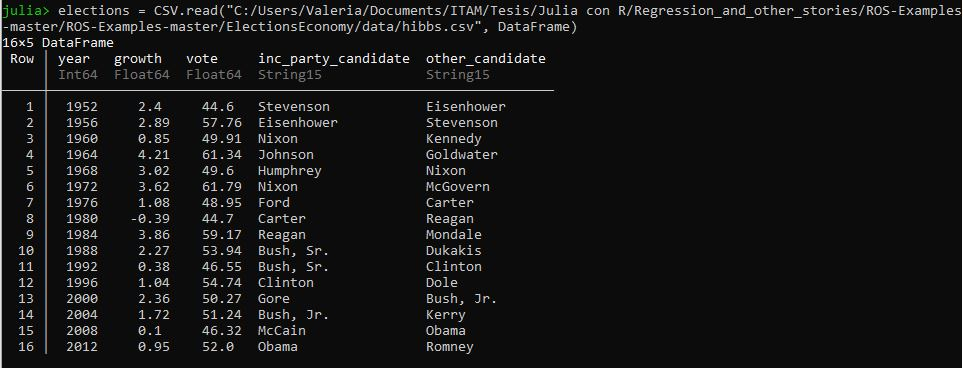
\includegraphics[scale=0.5]{Imagenes/elections_dataframe.JPG}
  \label{elections_dataframe}
\end{center}
\end{figure}

En este modelo busco que el voto sea resultado del crecimiento económico. El código para hacer esto en Julia es

\begin{minted}{julia}
	elections_lm = lm(@formula(vote ~ growth), elections)
\end{minted}

El resultado es una tabla con los coeficientes, la desviación estándar, el valor t, el valor p y el intervalo de confianza del $95 \% $ para los regresores. En este ejemplo, el resultado que da Julia es $y = 46.3 + 3.1x$ el cual coincide con los valores que da Gelman.

\subsubsection{Regresión lineal múltiple}

El caso general de la sección anterior se conoce como regresión lineal múltiple. La diferencia es que en este caso hay múltiples predictores que cumplen ciertos criterios. \cite{regression_other_stories} define este tipo de regresión como 

\begin{equation*}
    \begin{aligned}
    y_i = \beta_1 X_{i1} + \dots + \beta_k X_{ik} + \epsilon_i, \text{ para } i = 1, \dots, n
    \end{aligned}
\end{equation*}

donde los errores $\epsilon_i$ son independientes e idénticamente distribuidos de manera normal con media 0 y varianza $\sigma^2$. La representación matricial equivalente es 

\begin{equation} \label{eq_rlm}
    \begin{aligned}
        y_i = X_i \beta + \epsilon_i, \text{ para } i = 1, \dots, n
    \end{aligned}
\end{equation}

donde $X$ es una matriz de $n \times k$ con renglón $X_i$.

Para ejemplificar este tipo de modelo use un ejemplo que consta de dos predictores y la relación entre ellos. De nuevo utilicé los datos de \cite{regression_other_stories} que muestran la relación entre los resultados de exámenes de niños (\texttt{kid\_score}), el coeficiente intelectual IQ de sus madres (\texttt{mom\_iq}) y si sus madres terminaron o no la preparatoria (\texttt{mom\_hs}). 

Busco determinar si hay relación significativa entre la educación y el coeficiente de las madres con los resultados de exámenes de los niños. Por lo tanto, los predictores son las variables en relación con la madre mientras que la respuesta es el desempeño de los niños. El código en Julia se ve de la siguiente manera

\valinline{Como pongo el directorio de donde está mi base?}
\begin{minted}{julia}
    using DataFrames, GLM, CSV

    data_kid = CSV.read("C:/Users/Valeria/Documents/ITAM/Tesis/Julia con R/Regression_and_other_stories/ROS-Examples-master/ROS-Examples-master/KidIQ/data/kidiq.csv", DataFrame)

    fm = @formula(kid_score ~ mom_hs + mom_iq + mom_hs*mom_iq)

    kidscore_lm = lm(fm, data_kid)
\end{minted}

Lo cual da como resultado el modelo 

\begin{equation*}
    \begin{aligned}
        kid\_score = -11.48 + 51.26* mom\_hs + 0.97*mom\_iq \\
        -0.48*mom\_hs*mom\_iq + \epsilon
    \end{aligned}
\end{equation*}

Otro de los aspectos que hay que resaltar en este ejemplo es que para incluir la relación entre dos predictores basta usar un asterisco entre ellos al momento de definir la formula de la regresión. 

En el caso donde alguno de los regresores sea de tipo categórico la fórmula se mantiene igual pero hay que hacerle cambios a la base de datos en sí. Si Julia no reconoce estas columnas como categóricas entonces hay que cambiar su tipo en el dataframe. Abordo este problema más a fondo en el capítulo 8 \val{Checar al final que sí sea este capítulo}. Por otro lado, puedes intentar usar el paquete \texttt{CSVFiles} para leer los archivos ya que hace mejor trabajo identificando el tipo de variables. Sin embargo, este paquete todavía está en desarrollo por lo es más propenso a tener errores. 

\chapter{Python} \label{cap_python}

\say{Python es un lenguaje de programación que permite trabajar rápido e integrar sistemas más eficientemente} es una frase que podría parecer sencilla, pero es esa misma simplicidad la que la hace destacar como lo primero que se observa en la página oficial de \textsf{Python} \url{https://www.python.org/}. El creador de \textsf{Python}, Guido van Rossum, comenzó a desarrollar el lenguaje a finales de los ochentas para, finalmente, hacerlo público en 1991. Esto lo hace un lenguaje más antiguo que \textsf{Julia} y \textsf{R}. Sin embargo, su desarrollo y efectividad ha sido tal que empresas líderes mundiales en tecnología como Youtube y Google lo utilizan hoy en día. 

Los recursos de apoyo disponibles para el uso de \textsf{Python} son vastos y de todos los medios posibles. Se decidió incluirlo en este trabajo ya que su uso en ciencia de datos es cada vez más frecuente. Un ejemplo de ello es la publicación de libros escritos por reconocidos desarrolladores de software como lo son \textit{Python Data Science Handbook} de Jake VanderPlas y \textit{Python for Data Analysis} de Wes McKinney. Otros lenguajes de programación utilizados para ciencia de datos son \textsf{R, SQL} y \textsf{Stata}. 

\textsf{Python} se incluye también en este documento por su uso similar con \textsf{Julia} y \text{R} lo que permite mostrar su sencillez y facilidad de programación. En este trabajo se utilizó \textsf{Python} para los tres proyectos de manejo de datos que se explican a partir del capítulo \ref{cap_polinomios}. En dichos capítulos se presenta el código utilizado en los ejercicios, por lo que en las siguientes secciones se comentan los paquetes principales y la interfaz que se utilizaron. 

\section{Listas}
\say{Una \textit{lista} es una colección de elementos en un orden particular}, \cite{matthes2019python}. La lista es la estructura de datos elemental y principal de \textsf{Python} ya que permite almacenar diferentes tipos de elementos en un solo objeto. Una lista se crea usando paréntesis cuadrados \texttt{[]}. Por ejemplo, si se quisiera hacer una lista de animales en el zoológico el comando sería 

\begin{minted}{python}
animales = ["zebra", "leon", "jirafa", "elefante"]
animales[1]
\end{minted}

Los elementos de una lista pueden accederse mediante su índice y el uso de corchetes cuadrados. Por ejemplo, el comando \texttt{animales[1]} regresa \texttt{"león"}. Una característica clave de las listas en \textsf{Python} es que, a diferencia de \textsf{R} y \textsf{Julia}, las listas comienzan a numerar sus elementos desde el cero. 

Existen más estructuras de datos en \textsf{Python} cuyas características cumplen distintos criterios. En este trabajo se eligió trabajar con listas ya que son un objeto ordenado, mutable y que permite valores duplicados. Se recomienda ver la documentación de \textsf{Python}, \cite{doc_python}, para una explicación más detallada de los métodos propios de las listas. 

\section{Paquetes}
Al igual que en \textsf{Julia}, en \textsf{Python} se desarrolló el lenguaje original separado de los paquetes. La diversidad del desarrollo de los paquetes es tal que facilita hacer casi cualquier tipo de análisis matemático posible. 

Para usar cualquier instrucción de un paquete se tiene primero que nombrar su apodo y después llamar a la función. El apodo del paquete se lo otorga el usuario al momento de importarlo. Por ejemplo, 
\begin{minted}{python}
	import numpy as np
\end{minted}

\noindent importa el paquete \texttt{NumPy} con el apodo \texttt{np}. Si se quisiera llamar a la función \texttt{array} de este paquete se tendría que escribir el comando \texttt{np.array}. En las siguientes secciones se presentan los paquetes de \textsf{Python} utilizados en este trabajo. 

\subsection{NumPy} \label{seccion_numpy}
\texttt{NumPy} \citep{software_numpy} es el paquete fundamental para computación científica en \textsf{Python} ya que es el que proporciona los objetos multidimensionales como lo son los vectores y matrices. Estos objetos se pueden crear sin necesidad de \texttt{NumPy}, pero hacerlo mediante el paquete otorga algunas ventajas. La primera de ellas es que los arreglos creados en \texttt{NumPy} tienen dimensiones inmutables; la segunda es que sus elementos deben pertenecer del mismo tipo de dato; la tercera es que facilitan operaciones matemáticas en grandes cantidades de datos; y, finalmente, la cuarta es que es uno de los paquetes preferidos por la comunidad de \textsf{Python} lo cual lo hace objeto de una gran cantidad de publicaciones sobre su uso y aplicación. 

En esta tesis se usó \texttt{NumPy} para crear y manipular arreglos, así como hacer un ajuste de un polinomio usando el método de mínimos cuadrados. A continuación se presenta la lista completa de comandos que se utilizaron con su respectiva explicación proveniente del paquete oficial de \texttt{NumPy}, \cite{numpy_manual}. 

\begin{itemize}
	\item np.array([\texttt{lista}]): Crea un arreglo con los valores de la \texttt{lista}.
	
	\item np.insert(\texttt{arr, obj, values}): Inserta los valores \texttt{values} en el arreglo \texttt{arr} antes del índice \texttt{obj}.
	
	\item np.arange(\texttt{start, stop}): Crea un arreglo con valores espaciados uniformemente desde \texttt{start} hasta el número antes de \texttt{stop}. 
	
	\item np.transpose(\texttt{a}): Transpone el objeto \texttt{a}.
	
	\item np.concatenate(\texttt{$a_1, a_2, \dots $}): Une la secuencia de arreglos en uno ya existente.
	
	\item np.ones(\texttt{shape}): Crea una matriz de tamaño \texttt{shape} llena con unos.
	
	\item np.diag(\texttt{v}): Extrae la diagonal de la matriz \texttt{v} o crea una matriz diagonal de tamaño \texttt{v}.
	
	\item np.linalg.inv(\texttt{a}): Calcula la inversa multiplicativa de la matriz \texttt{v}. 
	
	\item np.random.choice(\texttt{a, size = None, replace = True, p = None}): Genera una muestra aleatoria de \texttt{a} de tamaño \texttt{size} con o sin reemplazo. 
	
	\item np.polyfit(\texttt{x, y, deg}): Hace un ajuste polinomial de grado \texttt{deg} a los puntos \texttt{(x, y)} usando el método de mínimos cuadrados. 
	
\end{itemize}


\subsection{pandas}
\texttt{pandas} \citep{software_pandas} es el segundo paquete en importancia de \textsf{Python} ya que ofrece manipulación y análisis de datos de manera rápida, flexible y sencilla. Sus funciones se enfocan en el uso eficiente de dataframes, lectura y escritura de datos, agrupación y unión de conjuntos de datos, entre otros \citep{pandas_manual}. En esta tesis se utilizaron los siguientes comandos de este paquete.

\begin{itemize}
	\item pd.read\_csv(\texttt{filepath}): Lee un archivo \texttt{csv} y lo convierte a dataframe.
	
	\item pd.DataFrame(\texttt{data}): Crea un objeto de tipo dataframe con los datos \texttt{data}. 
	
	\item pd.get\_dummies(\texttt{data}): Convierte las variables categóricas \texttt{data} en variables indicadoras o dummie. 
\end{itemize}

\subsection{os}
Otro módulo utilizado en este trabajo fue \texttt{os} \citep{software_python} ya que proporciona una manera portátil de usar la funcionalidad dependiente del sistema operativo \citep{doc_python}. Este es el paquete que permite hacer la conexión entre \textsf{Python} y los archivos de una computadora. Los comandos que se utilizaron son dos. El primero fue \texttt{os.chdir(path)} que permite seleccionar el directorio en el que se está trabajando. Mientras que el segundo fue \texttt{os.listdir(path)} que proporciona una lista de archivos en el \texttt{path} dado. 


\subsection{scikit-learn} \label{sec_sklearn}
\texttt{scikit-learn} \citep{software_scikitlearn} es un paquete creado para \textit{machine learning} o aprendizaje de máquina en \textsf{Python}. También es conocido como \texttt{sklearn} y proporciona herramientas simples y eficientes para la predicción en análisis de datos. Por ejemplo, clasificación, regresión, agrupamiento o conglomerado y reducción de dimensiones en modelos \citep{doc_python}. En este trabajo se utilizó para hacer regresiones lineales. El usuario puede importar el paquete de dos maneras. 

\begin{minted}{python}
	import sklearn
	from sklearn import linear_model
	
	regr = linear_model.LinearRegression()
	model = regr.fit(x, y)
\end{minted}

La primera línea de instrucción importa el paquete \texttt{sklearn} completo, mientras que la segunda solo toma la parte de modelos lineales. Con el paquete cargado, la tercera línea de código se encarga de guardar en la variable \texttt{regr} que lo que se busca es ajustar un modelo lineal definido como en la ecuación \ref{eq_rlm}. Finalmente, el último comando del código calcula los coeficientes $\beta$  usando el método de mínimos cuadrados. 

\subsection{itertools}
\say{itertools es un módulo que estandariza un conjunto importante de herramientas rápidas y eficientes de memoria que son útiles en sí mismas o en combinación}, \cite{doc_python}. Este paquete tiene ciertas funciones implementadas que se pueden recrear sin la necesidad del mismo. Sin embargo, la ventaja de utilizar \texttt{itertools} \citep{software_python} es la velocidad en la que las genera. 

En este trabajo se utilizo \texttt{itertools.combinations()} para crear las combinaciones de posibles factores activos del problema de discriminación de modelos presentado en el capítulo \ref{chapter_MDopt}. Todos los paquetes anteriores se utilizaron mediante la interfaz gráfica \textsf{Jupyter Notebook} que se presenta a continuación.

\section{Jupyter Notebook} \label{cap_jupyter}
\say{Jupyter Notebook es la aplicación web original para crear y compartir documentos computacionales. Es un programa que existe para desarrollar software de manera pública en decenas de lenguajes de programación incluyendo \textsf{R}, \textsf{Python} y \textsf{Julia}}, \cite{jupyter_page}. 

Una manera sencilla de obtener \textsf{Jupyter Notebook} es instalando \textsf{Anaconda}, una interfaz gráfica que permite manejar y administrar aplicaciones, paquetes, ambientes y canales sin necesidad de usar comandos en el sistema operativo. Para instalar Anaconda en \textsf{Windows} se debe ir a la página \url{https://docs.anaconda.com/anaconda/install/windows/} y seguir las instrucciones de instalación. Esto puede tomar unos minutos. Al terminar, la ejecución de \textsf{Jupyter Notebook} abrirá una ventana del explorador que se verá de manera similar a la imagen \ref{jupyter_pantallaPrincipal}. 


\begin{figure}[h]
	\begin{center}
		\includegraphics[scale=0.35]{Imagenes/jupyter_pantallaPrincipal.PNG}
		\caption{Pantalla principal de Jupyter Notebook}
		\label{jupyter_pantallaPrincipal}
	\end{center}
\end{figure}


\textsf{Jupyter Notebook} tiene la ventaja de facilitar el uso indistinto de los tres lenguajes utilizados en este trabajo. Uno de los prerequisitos para instalarlo es la instalación previa de \textsf{Python}. Por lo tanto, este es el lenguaje que ya viene en la interfaz. La figura \ref{pythonVersion} muestra, a manera de ejemplo, un archivo que utiliza \textsf{Python} en \textsf{Jupyter Notebook}. En la esquina superior derecha se puede verificar el lenguaje que se está utilizando. 

\begin{figure}[h]
	\begin{center}
		\includegraphics[scale=0.35]{Imagenes/pythonVersion.PNG}
		\caption{Archivo generado con Python en Jupyter Notebook}
		\label{pythonVersion}
	\end{center}
\end{figure}

El caso para \textsf{R} y \textsf{Julia} es diferente por lo que se expondrá su implementación en las siguientes secciones. 

\subsection{Julia}

El primer paso para utilizar \textsf{Julia} en la interfaz \textsf{Jupyter Notebook} es tener instalado el lenguaje en la computadora. Posteriormente, se debe instalar el paquete \texttt{IJulia} usando los pasos descritos en la sección \ref{instalacion_paquete}. Esto solo se tiene que hacer una vez. Para confirmar que la instalación esté bien hecha se debe abrir \textsf{Jupyter Notebook}, seleccionar \textsf{New} y debe aparecer la opción de \textsf{Julia 1.6.3} (o la versión de \textsf{Julia} que esté instalada en la computadora). El archivo nuevo generado con \textsf{Julia} se ve similar a la figura \ref{juliaVersion_ss}

\begin{figure}[h]
	\begin{center}
		\includegraphics[scale=0.35]{Imagenes/juliaVersion.PNG}
		\caption{Archivo generado con Julia en Jupyter}
		\label{juliaVersion_ss}
	\end{center}
\end{figure}

\subsection{R}

Existen varias maneras de instalar \textsf{R} en \textsf{Jupyter}, pero se expondrán los pasos descritos en el manual de \textsf{Anaconda}, \cite{anaconda_doc}. 

\begin{enumerate}
	\item Abrir el Navegador de \textsf{Anaconda} (no confundir con el de \textsf{Jupyter Notebook}).
	
	\item Seleccionar \texttt{Environments} y después la opción de \texttt{Create} ubicada en la esquina inferior izquierda. 
	
	\item Aparecerá una ventana donde permite al usuario nombrar el \texttt{Environment} como prefiera. Se debe seleccionar la versión de \textsf{Python} que se tenga y seleccionar la casilla del lado izquierdo de \textsf{R}. Después, se debe pulsar la opción de \texttt{Create}. 
	
	\item Para usar el ambiente que se acaba de crear en \textsf{Jupyter Notebook} se selecciona la flecha de lado derecho del nombre del ambiente nuevo. Entre las opciones seleccionar la opción de \texttt{Open with Jupyter Notebook} como se muestra en la figura \ref{abrirRconJupyter}
	
	\item Por último, se debe seleccionar el botón de \texttt{New} y después \textsf{R} para crear un archivo que trabaje con \textsf{R}. 
\end{enumerate}

\begin{figure}[h]
	\begin{center}
		\includegraphics[scale=0.35]{Imagenes/abrirRconJupyter.PNG}
		\caption{Ejecución de R desde el navegador de Anaconda}
		\label{abrirRconJupyter}
	\end{center}
\end{figure}

En la figura \ref{rVersion} se muestra el ejemplo de un archivo generado con \textsf{R} en \textsf{Jupyter Notebook}. En el siguiente capítulo se exponen las funciones utilizadas en \textsf{R}. 

\begin{figure}[h]
	\begin{center}
		\includegraphics[scale=0.35]{Imagenes/RVersion.PNG}
		\caption{Archivo generado con R en Jupyter Notebook}
		\label{rVersion}
	\end{center}
\end{figure}



\chapter{Ajuste de polinomios}

\section{El problema}
El problema que voy a abordar en esta sección es el mismo que abordaron \cite{laberintos} en el artículo mencionado en las referencias. Sin embargo, la diferencia es que yo utilicé Julia, R y Python  mientras que ellos compararon R, Excel, Stata, SPSS, SAS y Matlab. 

Supongamos que tenemos un conjunto de datos con solamente dos variables $x$, $y$. Buscamos ajustarlos a un polinomio de grado $k$. Es decir, buscamos ajustar los datos al modelo

\begin{equation*} 
    \begin{aligned}
    y = \sum_{j = 0}^{k} \beta_j x^j + \epsilon
    \end{aligned}
\end{equation*}

donde $j$ es el grado de la variable $x$. 

El problema consiste en encontrar los mejores coeficientes que cumplan la ecuación anterior. Una manera más compacta de ver el problema es de forma matricial 

\begin{equation}
\label{eq_matricial_pol}
    \begin{aligned}
    y = X \beta.
    \end{aligned}
\end{equation}

donde $y$ es un vector de tamaño $n$, $X$ es una matriz de tamaño $n \times (k + 1)$ y $\beta$ es un vector de tamaño $k + 1$. 


\section{Los datos}
En esta sección explicare como ajustar un conjunto de datos a un polinomio de grado $k$. Los datos que usare son proporcionados por el Instituto Nacional de Standards y Tecnología (NIST por sus siglas en inglés). Para este problema, seleccioné el conjunto llamado filip que se encuentra en \url{https://www.itl.nist.gov/div898/strd/lls/data/LINKS/DATA/Filip.dat}. Estos datos contienen 82 pares ordenados $(x_i, y_i)$. La siguiente imagen muestra las primeras 10 observaciones de los datos. 

\begin{figure}[h]
\begin{center}
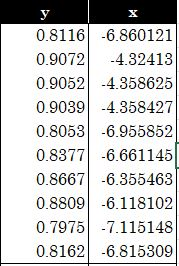
\includegraphics[scale=0.5]{Imagenes/header_filip.JPG}
  \label{header_filip}
\end{center}
\end{figure}

\valinline{no sé si agregar una gráfica rápida de los datos porque a simple vista no parecen un polinomio de grado 10}

Seleccioné este conjunto de datos porque además de proporcionar la información para el ajuste, también dan la respuesta al vector $\beta$ con alta precisión en sus dígitos. 

\section{Planteamiento del problema}

De esta forma, el vector $y$ de la ecuación \ref{eq_matricial_pol} es de tamaño 82 y corresponde a la columna $y$ del conjunto de datos.
Podríamos definir la matriz $X$ de la siguiente manera

\begin{equation*}
    \begin{aligned}
    X = 
    \begin{pmatrix}
    1 & x_{1,1} & x_{1,2} & \dots & x_{1, 10}  \\
    1 & x_{2,1} & x_{2, 2} & \dots & x_{2, 10} \\
    \vdots & \vdots & \vdots & \dots & \vdots \\
    1 & x_{81,1} & x_{81, 2} & \dots & x_{81, 10} \\
    1 & x_{82,1} & x_{82, 2} & \dots & x_{82, 10}. \\
    \end{pmatrix}
    \end{aligned}
\end{equation*} 

Representar la matriz $X$ de esta forma tiene una ventaja. Cada elemento puede ser visto como $x_{i, j}$ donde el renglón $i$ representa la observación $i$ de los datos. Por otro lado, la columna $j$ representa la potencia a la que está elevada la observación $i$. Por ejemplo, el elemento $x_{34, 5}$ es la observación 34 de los datos elevado a la 5 potencia. Sin embargo, es importante reconocer que el elemento $x_{34, 5}$ realmente está en la columna 6 de la matriz. El pequeño cambio de notación es solamente para no perder de vista la potencia de las observaciones. 


Por último, el vector $\beta$ de la ecuación \ref{eq_matricial_pol} es de dimensión 11 y es la incógnita del problema. 


En Julia, el código para cargar los datos es el siguiente: 

\begin{minted}{julia}
    using CSV, DataFrames, Polynomials
    
    filip = CSV.read("filip_data.csv", DataFrame)

    x = filip.x
    y = filip.y
    k = 10 #grado del polinomio
    n = length(x) # número de observaciones
\end{minted}

Por otro lado, para generar la matriz X creé una función que tiene como argumento una variable $k$ que representa la potencia del polinomio que quiero ajustar. 

\begin{minted}{julia}
function generar_X(k) # k es la potencia del polinomio

    n = size(filip, 1) #numero de renglones
    
    #Defino una matriz vacía
    X = Array{Float64}(undef, n, k + 1)
    # Sabemos que la primera columna siempre es un vector de unos
    X[:, 1] = ones(n)
    
    # Para el resto de la columnas,
    # elevo cada elemento a la potencia correspondiente
    for i = 1:k
        X[:, i + 1] = x.^i
    end
    return X
end
\end{minted}


\section{Métodos}

\subsection{\textit{GLM}}

Dado que el problema es ajustar una regresión lineal, el primer paquete que se viene a la mente por utilizar es \textsf{GLM}, ya que se sus siglas se traducen a 'Modelos Lineales Generalizados'.


El manual de este paquete se puede encontrar en \url{https://juliastats.org/GLM.jl/v0.11/#Methods-applied-to-fitted-models-1}. \val{No estoy segura si dejar esto o no} 

Para ajustar un modelo lineal generalizado, hay que utilizar la función \texttt{lm(formula, data)} donde 

\begin{itemize}
    \item formula: 
    Corresponde a la fórmula del ajuste con los nombres de las columnas de los datos
    \item data:
    Debe ser un dataframe con los datos por ajustar. Los datos pueden contener valores NA. 
\end{itemize}

En nuestro caso, queremos ajustar un polinomio de grado 10 a los datos guardados con el nombre de filip. Por lo tanto, el código en Julia es

\begin{minted}{julia}
    x_fit = lm(@formula(y ~ 1 + poly(x, 10)), filip)
\end{minted}

donde \texttt{poly(x, 10)} es una función con sintaxis extendida que se utiliza específicamente para regresión polinomial. Esta función viene programada en la documentación del paquete \textsf{StatsModels} en el apartado de \textsf{Extending @formula syntax} que se encuentra en la dirección \url{https://juliastats.org/StatsModels.jl/stable/internals/}. \val{No sé si mejor poner la referencia?? creo que si}



Este método no funcionó. Dado que los datos de NIST vienen con la respuesta correcta, fue claro observar que los resultados con el paquete GLM no ajustaron de manera precisa el polinomio. 

\subsection{Descomposición QR versión económica}

\begin{definition}
La factorización QR de una matriz $A$ de dimensiones $m \times n$ es el producto de una matriz $Q$ de $m \times n$ con columnas ortogonales y una matriz $R$ cuadrada y triangular superior \cite[p.~191]{garcia2017second}. 
\end{definition}

Una de las aplicaciones de la descomposición QR es dar solución a problemas de mínimos cuadrados. Por lo tanto, es el segundo método que utilizamos para obtener los valores $\beta$ de \ref{eq_matricial_pol}.

 \begin{definition}
 Una secuencia de vectores $u_1, u_2, \dots$ (finita o infinita) en un espacio de producto interno es ortonormal si 
 \begin{equation*}
     \begin{aligned}
     \langle u_i , uj \rangle = \delta_{ij} \text{ para toda $i, j$}
     \end{aligned}
 \end{equation*}
 Una secuencia ortonormal de vectores es un sistema ortonormal \cite[p.~147]{garcia2017second}.
 \end{definition}

\begin{definition}
Una base ortonormal para un espacio de producto interno finito es una base que es un sistema ortonormal \cite[p.~149]{garcia2017second}.
\end{definition}

En nuestro problema las dimensiones $m \times n$ de la matriz $X$ son $82 \times 11$. Además, $X$ tiene rango $r = 10 < n$ por lo que la matriz $R$ de la descomposición QR es singular. Como consecuencia, no se puede generar una base ortonormal de $R(X)$. Sin embargo, el proceso de factorización QR se puede modificar usando una matriz de permutación para generar una base ortonormal.


\begin{definition}
Una matriz $A$ es una matriz de permutación si exactamente una entrada en cada renglón y en calada columna es 1 y todas las otras entradas son 0 \cite[p.~183]{garcia2017second}.
\end{definition}

La idea del método QR modificado es generar una matriz de permutación $P$ tal que 

\begin{equation*}
    \begin{aligned}
    AP = QR
    \end{aligned}
\end{equation*}

donde 

\begin{equation*}
    \begin{aligned}
    R = 
    \begin{pmatrix}
    R_{11} & R_{12} \\
    0      & 0
    \end{pmatrix}
    \end{aligned}
\end{equation*}

En este caso, si tomamos $r$ como el rango de $X$ entonces $R_{11}$ es de dimensión $r \times r$ triangular superior y $Q$ es ortogonal. Las primeras $r$ columnas de $Q$ forman una base ortonormal de $R(X)$ \cite{numerical_linear_algebra}. La factorización QR con columnas pivoteadas \val{si se dice asi? le dicen version economica en el articulo pero no encuentro la traduccion} siempre existe debido al siguiente teorema.

\begin{theorem} \label{exitencia_QR_dec}
Sea $A$ una matriz de $m \times n$ con rango($A$) = $r \leq min (m, n)$. Entonces, existe una matriz de permutación $P$ de $n \times n$ y una matriz ortogonal $Q$ de dimensiones $m \times m$ tal que 
\begin{equation*}
\begin{aligned}
Q^{T}AP = 
\begin{pmatrix}
R_{11} & R_{12} \\
   0      & 0
\end{pmatrix}
\end{aligned}
\end{equation*}
donde $R_{11}$ es una matriz triangular superior de tamaño $r \times r$ con entradas en la diagonal diferentes de cero \cite[p.~532]{numerical_linear_algebra}.
\end{theorem}

\val{literal el teorema viene de Datta 2010}

Para aplicar este método en Julia, hay que usar el siguiente código

\begin{minted}{julia}
    ### Con QR Pivoted
    F = qr(X, Val(true))
    Q = F.Q
    P = F.P
    R = F.R
\end{minted}



Ya tenemos el código que calcula las matrices $P, Q, R$ de la descomposición QR con columnas pivoteadas. Para resolver nuestro problema original \ref{eq_matricial_pol} y obtener los valores de los elementos de $\beta$ hay que hacer un poco de álgebra. 



Recordemos que el problema es obtener $\beta$ de la ecuación $y = X \beta$. También, por el teorema \ref{exitencia_QR_dec}, sabemos que $X$ siempre tiene descomposición QR con columnas pivoteadas. Es decir, $XP = QR$. Por otro lado, como $P$ es matriz de permutación por lo que

\begin{equation*}
    \begin{aligned}
    \exists z \text{ tal que } Pz = \beta .
    \end{aligned}
\end{equation*}

Por lo tanto, ya tenemos una expresión para $\beta$ que podemos sustituir en la ecuación \ref{eq_matricial_pol} para obtener 
\begin{equation*}
    \begin{aligned}
    y = X (Pz) . 
    \end{aligned}
\end{equation*}

A la vez, sustituyendo en la fórmula de la descomposición QR

\begin{equation*}
    \begin{aligned}
    (XP) z = (QR) z . 
    \end{aligned}
\end{equation*}

Uniendo las dos ecuaciones anteriores, obtenemos 

\begin{equation*}
    \begin{aligned}
    y = XP z = QR z 
    \longrightarrow y = QRz
    \end{aligned}
\end{equation*}

Por lo tanto, el primer paso es resolver la ecuación 

\begin{equation*}
    \begin{aligned}
    y = QRz
    \end{aligned}
\end{equation*}

Para finalmente obtener $\beta$ calculando 
\begin{equation*}
    \begin{aligned}
    \beta = Pz
    \end{aligned}
\end{equation*}

En Julia, esto se programa de la siguiente manera
\begin{minted}{julia}
    # 1. Resolver QRz = y
    z = Q*R \ y
    # 2. Resuelvo beta = Pz
    x_QR = P*z
\end{minted}


Este método tampoco funcionó. Podemos empezar a consider que los datos son tan sensibles que la propagación del error es tal que no permite un buen ajuste del polinomio. Intentaremos con otros dos métodos.

\subsection{Descomposición de valores singulares}

La tercer manera en la que intenté resolver este problema fue usando la descomposición de valores singulares para obtener la matriz pseudoinversa de Moore-Penrose. 

\begin{definition}
Sea $A$ una matriz de $m \times n$ y sea $q = min \{m, n \}$. Si el rango de $A = r \geq 1$, sean $\sigma_1 \geq \sigma_2 \geq \dots \geq \sigma_r > 0$ los eigenvalores positivos en orden decreciente de $(A^{*}A)^{1/2}$. Los valores singulares de $A$ son
\begin{equation*}
    \begin{aligned}
    \sigma_1, \sigma_2, \dots, \sigma_r \text{ y } \sigma_{r+1} = \sigma_{r+2} = \dots = \sigma_q = 0.
    \end{aligned}
\end{equation*}
Si A = 0, entonces los valores singulares de A son $\sigma_1 = \sigma_2 = \dots = \sigma_q = 0$. 
Los valores singulares de $A \in M_{n}$ son los eigenvalores de $(A^{*}A)^{1/2}$ que son los mismos eignevalores de $(AA^{*})^{1/2}$
\cite[p.~420]{garcia2017second}
\end{definition}

Los valores singulares tienen muchas apliciones. Sin embargo, para resolver ecuaciones lineales son usados para obtener la descomposición de valores singulares (DVS). 


\begin{theorem}
Sea $A \in M_{m \times n} (F)$ diferente de cero y sea $r =   rango(A)$. Sean $\sigma_1 \geq \sigma_2 \geq \dots \geq \sigma_r > 0$ los valores singulares positivos de A y definamos

\begin{equation*}
    \begin{aligned}
    \Sigma_r = 
    \begin{pmatrix}
    \sigma_1 & & 0 \\
     & \ddots & & \\
     0 & & \sigma_r
    \end{pmatrix}
    \in M_{r}(R).
    \end{aligned}
\end{equation*}
Entonces, existen matrices unitarias $U \in M_{m}(F)$ y $V \in M_{n}(F)$ tales que 
\begin{equation} \label{decomposicion}
    \begin{aligned}
    A = U \Sigma V^{*}
    \end{aligned}
\end{equation}
donde
\begin{equation*}
    \begin{aligned}
    \Sigma = 
    \begin{pmatrix}
    \Sigma_r & 0_{r \times (n-r)} \\
    0_{(m-r) \times r} & 0_{(m-r) \times (n-r)}
    \end{pmatrix}
    \in M_{m \times n}(R)
    \end{aligned}
\end{equation*}
 tiene las mismas dimensiones que A. Si m = n, entonces $U, V \in M_{n}(F)$ y $\Sigma = \Sigma_r \oplus 0_{n-r}$.
 \cite[p.~421]{garcia2017second}
\end{theorem}

La ecuación \ref{decomposicion} con las características del teorema anterior lleva por nombre descomposición en valores singulares (DVS). 


Es importante observar que las matrices $U$ y $V$ son matrices unitarias. Es decir, 

\begin{equation*}
    \begin{aligned}
    U U^{*} u = u, \text{ } \forall u \in Col (U)
    \end{aligned}
\end{equation*}

\begin{equation*}
    \begin{aligned}
    V V^{*} v = v, \text{ } \forall v \in Col (V)
    \end{aligned}
\end{equation*}

\subsubsection{Pseudoinversa de Moore-Penrose}

Ya que conocemos la descomposición de valores singulares, podemos avanzar y definir la descomposición de valores singulares para la pseudoinversa de Moore Penrose. 

\begin{theorem}
Sea $A$ una matriz de $m \times n$ de rango $r$ con una descomposición en valores singulares de $A = U \Sigma V^{*}$ y valores singulares diferentes de cero $\sigma_1 \geq \sigma_2 \geq \dots \geq \sigma_r$. Sea $\Sigma^{\dagger}$ una matriz de $n \times m$ definida como
\begin{equation*}
    \begin{aligned}
   \Sigma^{\dagger}_{ij} =
   \begin{cases}
   \dfrac{1}{\sigma_i} \text{ si } i = j \leq r\\
   0 \text{ en otro caso.}
   \end{cases}
    \end{aligned}
\end{equation*}
Entonces $A^{\dagger} = V \Sigma^{\dagger} U ^{*}$ y esta es la descomposición de valores singulares de $A^{\dagger}$. 
\cite[p.~414]{friedberglinearalgebra}
\end{theorem}

Podemos ver que en realidad lo único que cambia al calcular la pseudoinversa es la matriz $\Sigma$. Sin embargo, esta nueva matriz $A^{\dagger}$ tiene propiedades interesantes. 

\begin{itemize}
    \item $(A^{T}A)^{\dagger} A^{T} = A^{\dagger}$
    \item $(AA^{T})^{\dagger} A = (A^{\dagger})^{T}$
    \item $(A^{T}A)^{\dagger}(A^{T}A) = A^{\dagger}A = VV^{T}$
\end{itemize}


Recordando que buscamos obtener $\beta$ que satisfaga la ecuación \ref{eq_matricial_pol} podemos ver que el sistema lineal está sobredeterminado. Esto se puede verificar por las dimensiones de la matriz $X_{n \times m} = X_{82 \times 11}$. Como $m < n$, sabemos que hay más ecuaciones que variables desconocidas. 


\valinline{Como sabemos que y esta en el espacio de columnas de V?}
De la ecuación \ref{eq_matricial_pol} podemos multiplicar por $X^{T}$ para obtener
\begin{equation}
\label{transformacion_eq_base}
    \begin{aligned}
    X^{T}X \beta = X^{T} y, \text{ } y \in Col(V).
    \end{aligned}
\end{equation}

La ecuación \ref{transformacion_eq_base} siempre da un sistema determinado (balanceado) \cite{worldScientificNews}. Ahora bien, multiplicando \ref{transformacion_eq_base} por $(X^{T}X)^{\dagger}$ y usando las propiedades de la matriz pseudo inversa podemos obtener 


\begin{equation*}
    \begin{aligned}
    (X^{T}X)^{\dagger} X^{T}X \beta = (X^{T}X)^{\dagger} X^{T} y \\
    \iff X^{\dagger} X \beta = X^{\dagger} y \\
    \iff V V^{T} \beta = X^{\dagger} y \\
    \beta = X^{\dagger} y 
    \end{aligned}
\end{equation*}. 

Por lo tanto, la pseudo inversa de Moore Penrose da la solución de mínimos cuadrados de \ref{eq_matricial_pol} \cite{worldScientificNews}


En Julia, este método se puede programar de la siguiente manera:

\begin{minted}{julia}
    # # # Inversa de Moore Penrose
    N = pinv(X)
    aux = ones(k + 1)
    x_MP = N*y 
\end{minted}

Este método tampoco funcionó. Por lo tanto, investigue más a fondo los paquetes de Julia hasta encontrar el paquete \textit{Polynomials}. 

\subsection{\textit{Polynomials}}
\textit{Polynomials} es un paquete que proporciona aritmética básica, integración, diferenciación, evaluación y hallar raíces para polinomios univariados \cite{poly_manual}. Para poder usar el paquete primero hay que descargarlo usando el código \ref{instalacion_paquete}. 


El paquete \textit{Polynomials} tiene su propia función \texttt{fit} que toma tres variables como entrada. Las primeras dos entradas son las correspondientes a $x$ y $y$ de los datos a utilizar (en este caso, los datos filip). La tercera entrada corresponde al grado que buscamos que sea el polinomio (en este caso, grado 10). 

A diferencia de los otros método utilizados para este problema, la función \texttt{fit} usa el metódo Gauss-Newton para resolver sistemas de ecuaciones no lineales. Sin embargo, en este caso tenemos un problema lineal. Esta fue la primera razón por la que este paquete no fue mi primera opción para resolver el problema. 
\valinline{No sé si tengo que explicar este método}


La segunda razón es que a diferencia de la función \texttt{lm} del paquete \textit{GLM}, la función \texttt{fit} solamente aporta los coeficientes del ajuste del polinomio. Es decir, no da como resultado el error estandar, ni el valor p de la estimación. Sin embargo, tengo que agregarlo a esta sección de la tesis, ya que es el único método que funcionó. 


El código en Julia se ve de la siguiente manera:

\begin{minted}{julia}
using Polynomials 
x_pol = Polynomials.fit(x, y, 10)
\end{minted}


Este método fue el único de los cuatro que funcionó para el polinomio de grado 10. La desventaja de este método es que la función solamente arroja los coeficientes $\beta$. Si quisieramos ampliar el análisis y observar, por ejemplo, el valor p de algún regresor tendríamos que buscar otra manera de obtenerlo. 


\section{Evaluación de los métodos}
Una cuestión válida es preguntarse si tal vez lo que está mal es la implementación de los algoritmos y, debido a esto, no dan la respuesta correcta. Por tanto, para probar que los métodos estén programados de la manera correcta los somentí a una serie de pruebas.


La primera prueba consiste en que, usando los datos filip, cada método ajustaba un polinomio de grado $k$ de $k = 1, 2, \dots, 10$. Al final, para cada polinomio de grado $k$ tenía cuatro resultados de ajuste (uno por cada método). 

La segunda prueba consiste en comparar los resultados con R. De manera análoga a Julia, en R también use los datos filip para ajustar un polinomio de grado $k$ de $k = 1, 2, \dots, 10$. Para esto, use la función \texttt{lm(formula, data)} donde los datos siempre son los mismos y la fórmula depende del grado del polinomio. Es importante mencionar que este problema ya ha sido abordado por otros usuarios y resuelto por Brian Ripley. Ripley es un matemático británico que ha escrito muchos libros sobre programación y ha ganado muchos premios por sus aportaciones a la estadística. Sin duda lo más relevante en este caso es que es uno de los contribuidores principales en el desarrollo de \textsf{R}. El código que utilicé para resolver este problema es el mismo que Ripley hizo público. 


La tercera prueba fue medir el tiempo que tomaba a R ejecutar la función \texttt{lm} con los parametros especificados. El código es el siguiente: 

\begin{minted} {R}
# Para polinomio de grado = 1
start <- Sys.time()
lm_1 <- lm(y ~ x, data = data, x = TRUE)
end <- Sys.time()

`resultados_grado_ 1`$R <- lm_1$coefficients
row.names(`resultados_grado_ 1`) <- c("b0", "b1")
X_1 <- lm_1$x

time_vec <- c(end - start)

# Para polinomios de grado > 1

for (i in 2:10){
  #Hacemos el modelo
  model <- paste("y ~ x", paste("+ I(x^", 2:i, ")", sep='', collapse=''))
  
  # Lo convertimos en formula
  form <- formula(model)
  
  #Ejecutamos el modelo
  start <- Sys.time()
  lm.plus <- lm(form, data = data, x = TRUE)
  end <- Sys.time()
  time <- end - start
  time_vec <- c(time_vec, time)
  
  # Guardo el df correspondiente a un auxiliar
  resultados_aux <- get(paste("resultados_grado_", i))
  # para unirle los coeficientes
  resultados_aux$R <- lm.plus$coefficients
  
  nombres <- c("b0")
  # Para el nombre de los renglones
  for (k in 1:i){
    nombres <- c(nombres, paste0("b", k))
  }
  row.names(resultados_aux) <- nombres
  
  #Finalmente, hago el df final
  assign(paste("resultados_grado_", i), resultados_aux)
  
  assign(paste("X_", i), lm.plus$x)
 
\end{minted}

No voy a mostrar todas las tablas con los resultados ya que son muchas. Me voy a limitar a las tablas que considero tienen los resultados más relevantes. Para el polinomio de grado 1, todos los métodos obtienen los mismos resultados. 

\begin{figure}[h]
\begin{center}
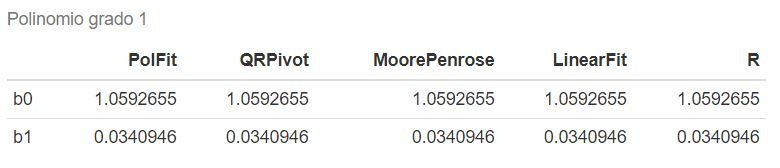
\includegraphics[scale=0.5]{Imagenes/tabla_pol_1.JPG}
\end{center}
\end{figure}

Todos los métodos funcionan bien calculando el ajuste hasta llegar al polinomio de grado 5. Cuando calculamos el polinomio de grado 6, el método \texttt{fit} del paquete \texttt{GLM} llamado \texttt{LinearFit} comienza a fallar. 

\begin{figure}[h]
\begin{center}
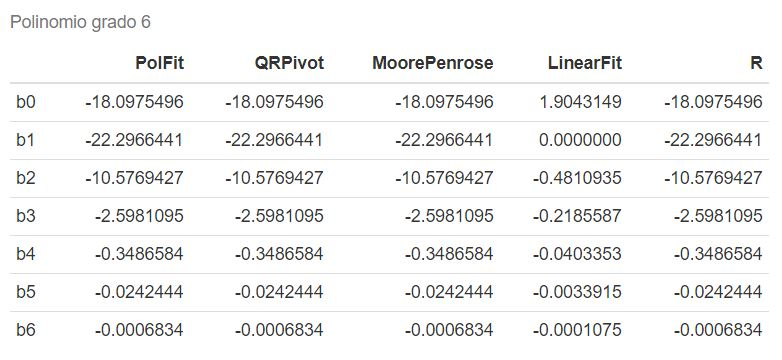
\includegraphics[scale=0.5]{Imagenes/tabla_pol_6.JPG}
\end{center}
\end{figure}

A partir del polinomio de grado 6, \texttt{LinearFit} comienza a fallar y comienza a dar resultados muy érroneos. Todos los métodos arrojan resultados correctos hasta que llegamos al polinomio de grado 10. 

\begin{figure}[h]
\begin{center}
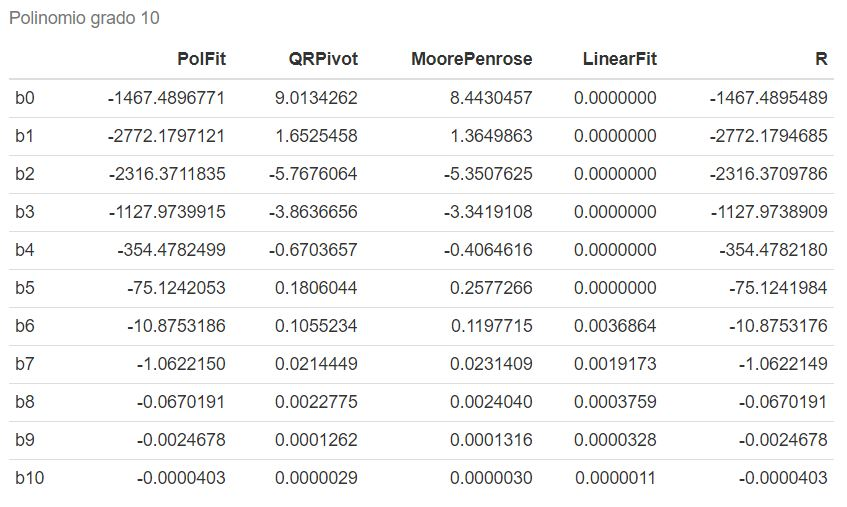
\includegraphics[scale=0.5]{Imagenes/tabla_pol_10.JPG}
\end{center}
\end{figure}

Finalmente, podemos ver la tabla de tiempos que le tomo a cada método. Las columnas representan los métodos usados mientras que los renglones el grado de polinomio que se ajustó. 

\begin{figure}[h]
\begin{center}
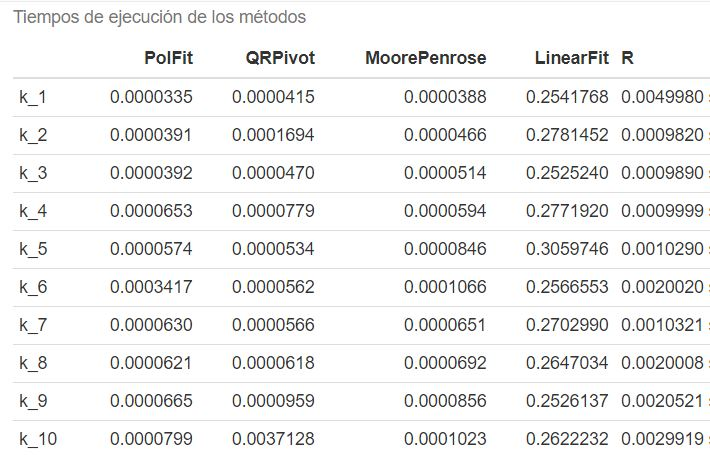
\includegraphics[scale=0.5]{Imagenes/table_tiempos.JPG}
\end{center}
\end{figure}

\valinline{Las tablas están por donde quieren, mejor copio los resultados?}



\section{Eigenvalores y valores singulares}
\valinline{No estoy segura de que poner dado que no sale la igualdad basica entre eigenvalores y valores singulares}

\section{Número de condición y precisión de la solución}

\begin{definition}
El número $\parallel A \parallel  \parallel A^{-1} \parallel$ se llama el número de condición de $A$ y se denota $Cond(A)$ \cite[p.~62]{numerical_linear_algebra}. 
\end{definition}

Como vimos en la sección de Evaluación de los métodos, los métodos sí están bien programados. Dejando de lado las funciones programadas por default en Julia, el método de factorización QR y descomposición de valores singulares arrojaron buenos resultados hasta los polinomios de grado 9. Esto nos puede llevar a pensar que en realidad, los datos en sí son muy susceptibles a cambios. Es decir, cualquier cambio en la matriz $X$ o en el vector $y$ resultara en un ajuste de los coeficientes $\beta$ poco preciso. Esta cualidad también se conoce como que los datos tienen impurezas. El caso contrario, donde los métodos dan resultados precisos se conoce a los datos como exactos \cite{numerical_linear_algebra}.


En general, para nuestro problema \ref{eq_matricial_pol} tenemos tres casos: 
\begin{itemize}
    \item El vector $y$ tiene impurezas mientras que la matriz $X$ es exacta. 
    \item La matriz $X$ tiene impurezas mientras que el vector $y$ es exacto
    \item Ambos, el vector $y$ y la matriz $X$ tiene impurezas. 
\end{itemize}

En nuestro caso, nos vamos a enfocar en el tercer caso ya que no tenemos razón para pensar que solamente una columna de los datos originales tiene impurezas mientras que la otra no. 


\begin{theorem} \label{teo:perturbaciones}
Supongamos que queremos resolver el sistema $Ax = b$. Supongamos que $A$ es no singular, $b \neq 0$, y $\parallel \Delta A \parallel < \dfrac{1}{\parallel A^{-1} \parallel}$. Entonces
\begin{equation*}
    \begin{aligned}
    \dfrac{\parallel \delta x \parallel}{\parallel x \parallel} \leq (\dfrac{Cond(A)}{1 - Cond(A) \dfrac{\parallel \Delta A \parallel}{\parallel A \parallel}}) (\dfrac{\parallel \Delta A \parallel}{\parallel A \parallel} + \dfrac{\parallel \delta b \parallel}{\parallel b \parallel})
    \end{aligned}
\end{equation*} \cite[p.~65]{numerical_linear_algebra}
\end{theorem}

El teorema anterior nos está diciendo que los cambios en la solución $x$ son menor o iguales a una constante determinada por el número de condición multiplicada por la suma de las pertubaciones de $A$ y las pertubaciones de $b$. Además, el teorema nos dice que aunque las perturbaciones de $A$ y $b$ son pequeñas, puede haber un cambio grande en la solución si el número de condición es grande. Por lo tanto, $Cond(A)$ juega un papel crucial en la sensibilidad de la solución \cite{numerical_linear_algebra}. 


El número de condición tiene varias propiedades pero en la que nos queremos centrar es en la siguiente: 

\begin{equation} \label{formula:num_cond}
    \begin{aligned}
    Cond(A) = \dfrac{\sigma_{max}}{\sigma_{min}}
    \end{aligned}
\end{equation}

donde $\sigma_{max}$ y $\sigma_{min}$ son, respectivamente, el valor singular más grande y más pequeño de $A$. 

Antes de calcular el número de condición de nuestra matriz $X$ de \ref{eq_matricial_pol}, vamos a ver una última definición. 

\begin{definition} \label{def:condicionamiento}
El sistema $Ax = b$ está mal condicionado si el $Cond(A)$ es grande (por ejemplo, $10^{5}, 10^{8}, 10^{10}, etc)$. En otro caso, está bien condicionado \cite[p.~68]{numerical_linear_algebra}.
\end{definition}

Ahora vamos a calcular el número de condición. Este calculo lo hice en Julia y en R usando ambos, la función que ya viene programada en cada lenguaje y usando la fórmula \ref{formula:num_cond}. En Julia, el código es 

\begin{minted}{julia}
# Con función de Julia
numcond_1 = cond(X_10)

# Usando propiedad de valores singulares
sing_values = svd(X_10).S
sing_values = sort(sing_values)
numcond_2 = sing_values[length(sing_values)] / sing_values[1]
\end{minted}

Los resultados son $numcond_1 = 1.7679692504686805e15$ y $numcond_2 = 1.7679692504686795e15$. Por otro lado, en R el código es 

\begin{minted}{R}
# con función de R
numcond_R1 <- cond(X)

# Usando propiedad de valores singulares
S.svd <- svd(X)
S.d <- S.svd$d
S.d <- sort(S.d, decreasing = TRUE)
numcond_R2 <- S.d[1] / S.d[length(S.d)]
\end{minted}

Los resultados son $numcond_{R1} = numcond_{R2} = 1.767962e{15}$. En conclusión, en ambos lenguajes cualquier método confirma que el número de condición de la matriz $X$ de \ref{eq_matricial_pol} es bastante grande por lo que por \ref{def:condicionamiento} sabemos que nuestro problema está mal condicionado. \valinline{Tengo duda, entonces alguien me podría decir que para que los uso}








\chapter{Regresión Lineal Múltiple}

\section{El problema}
En esta sección veremos como hacer una regresión lineal múltiple usando Julia. El modelo de regresión lineal clásico es 

\valinline{No se porque no sale el beta 0}

\begin{equation} \label{rlm_eq}
    \begin{aligned}
    y_i = \beta_i X_{i1} + \dots + \beta_k X_{ik} + \epsilon_i \text{, para } i = 1, \dots, n \text{ \cite[p.~146]{regression_other_stories}}
    \end{aligned}
\end{equation}

donde los errores son independientes y siguen una distribución normal con media 0 y desviación estándar $\sigma$. En este caso, $y_i$ se refiere al nivel i-ésimo del regresor; $x_{ij}$ es el j-ésimo regresor al i-ésimo nivel; y $\beta_j$ es el coeficiente del j-ésimo regresor. \val{Esto es de las notas del profesor Barrios}


De manera matricial, la ecuación \ref{rlm_eq} se puede escribir como \begin{equation*}
    \begin{aligned}
    y_i = X_i \beta + \epsilon_i \text{, para } i = 1, \dots, n
    \text{ \cite[p.~146]{regression_other_stories}}
    \end{aligned}
\end{equation*}

donde $X$ es una matriz de $n \times k$ donde su i-ésimo renglón es $X_i$. 

\section{Los datos}
Tomando en cuenta que los modelos estadísticos se utilizan como un reflejo de la realidad decidí usa los datos del Censo de Población y Vivienda 2020. Los datos son publicados por el Instituto Nacional de Estadística y Geografía (INEGI) y se pueden encontrar en la página \url{https://www.inegi.org.mx/programas/ccpv/2020/default.html}. 


El propósito del Censo 2020 es producir información sobre el volumen, la estructura y la distribución espacial de la población, así como de sus principales características demográficas, socioeconómicas y culturales; además de obtener la cuenta de las viviendas y sus características tales como los materiales de construcción, servicios y equipamiento, entre otros \val{agregar referencia de la página del INEGI}. Los resultados del Censo que estoy utilizando vienen de las respuestas al llamado cuestionario ampliado cuyas 103 preguntas resultan en alrededor de 200 variables de estudio. Asimismo, el Censo fue aplicado a 4 millones de viviendas a lo largo de la República Mexicana que dio resultado a la obtención de información de más de 15 millones de personas.

En este caso, elegí un tema que es de interés para todos los adultos: los ingresos. Más específicamente, quiero usar la RLM para ver como afectan diferentes variables al ingreso de cada persona. Usualmente, es trabajo del estadístico construir un modelo desde cero usando una combinación de lógica, referencias y experiencia. En este caso, el modelo final que ajusté es 
\begin{equation} \label{modelo_final}
    \begin{aligned}
    ingresos \sim horas_{trabajadas} + sexo + edad + escolaridad + entidad_{residencia} + \\ posicion_{laboral} + alfabetismo + aguinaldo + vacaciones + servicio_{medico}
    \end{aligned}
\end{equation}


\section{Planteamiento del problema}
El Censo es el conjunto de cuestionarios que se le aplican a distintas personas en México. Por eso, antes de comenzar a ajustar los datos, hay que hacer un filtro. Para hacer este filtro y saber que significa cada variable así como sus posibles respuestas, descargué el diccionario del cuestionario ampliado que se encuentra en \url{https://www.inegi.org.mx/programas/ccpv/2020/default.html#Microdatos} dentro del apartado \textsf{Documentación de la base de datos}. El diccionario es de suma importancia ya que proporciona el significado de los códigos que usaron para pasar las respuestas de una hoja de papel a una base de datos. 


La información de los resultados del Censo está dividida en tres partes: Viviendas, Personas y Migrantes. En esta ocasión, utilicé solamente la base de datos de Personas ya que contiene toda la información que necesito. 


La cantidad de datos con la que estoy trabajando es enorme por lo que en primer lugar seleccione solamente las columnas que necesito. Después, puse los siguientes filtros 

\begin{enumerate}
    \item 
    \item Obtuve solamente las personas tienen un trabajo remunerado. Es decir, no consideré las personas que
    se ocupan de las labores del hogar, son jubiladas o pensionadas, son estudiantes o tienen alguna incapacidad que les impide trabajar. 
    
    \item Descarté a las personas que viven y trabajan fuera de la República Mexicana. 
    
    \item Obtuve solamente a las personas que especificaron horas trabajadas e ingreso ganado.
    
    \item Además, para las variables que representan los regresores quité a todas las personas que respondieron a alguna de esas preguntas con \textsf{No específicado}. 
\end{enumerate}

Finalmente, ya que la base se reduce considerablemente y todo el proceso dura alredodr de 20 minutos en efectuarse guardo la nueva base de datos filtrada para en un futuro solamente leerla y utilizarla. Al final, el código queda de la siguiente manera.

\begin{minted}{julia}
using CSV, DataFrames, StatsBase, GLM, Random, CategoricalArrays

# Equivalente a set.seed
Random.seed!(99)

#Leer la base de datos (toma alrededor de 4 minutos en cargar)
personas = CSV.read("Personas00.csv", DataFrame)

# Las columnas que estoy seleccionando para el ajuste
col_sel = ["ID_PERSONA","ENT","SEXO", "EDAD", "NIVACAD", "ALFABET", 
            "INGTRMEN","HORTRA", "CONACT", "SITTRA", "ENT_PAIS_TRAB",
        "AGUINALDO", "VACACIONES", "SERVICIO_MEDICO", "UTILIDADES", "INCAP_SUELDO", "SAR_AFORE", "CREDITO_VIVIENDA"]
# Selecciono solo las columnas del ajuste
personas_filt = personas[:, col_sel]    

# # # FILTRO 1
cond_act = [10, 13, 14, 15, 16, 17, 18, 19, 20]
personas_filt = subset(personas_filt, :CONACT => ByRow(in(cond_act)), skipmissing = true)

# # # FILTRO 2
personas_filt = subset(personas_filt, :ENT_PAIS_TRAB => ByRow(<(33)), skipmissing = true)

personas_filt = subset(personas_filt, :ENT => ByRow(<(33)), skipmissing = true)

# # # FILTRO 3
personas_filt = subset(personas_filt, :HORTRA => ByRow(!=(999)), skipmissing = true)

personas_filt = subset(personas_filt, :INGTRMEN => ByRow(!=(999999)), skipmissing = true)

# # # FILTRO 4
function diferente_a(dataframe, columna, condicion)
    dataframe = subset(dataframe, columna => ByRow(!=(condicion)), skipmissing = true)
    return dataframe
end

categorias_9 = ["SEXO", "AGUINALDO", "VACACIONES", "SERVICIO_MEDICO", "UTILIDADES", 
    "INCAP_SUELDO", "SAR_AFORE", "CREDITO_VIVIENDA", "ALFABET", "SITTRA"]

categorias_99 = ["NIVACAD"]

for i = 1:length(categorias_9)
    personas_filt = diferente_a(personas_filt, categorias_9[i], 9)
end

for i = 1:length(categorias_99)
    personas_filt = diferente_a(personas_filt, categorias_99[i], 99)
end

# Finalmente, guardo el nuevo dataframe
CSV.write("personas_filtradas.csv", personas_filt)
\end{minted}


\section{Regresiones}
\valinline{No estoy segura de como ponerle de nombre a esta seccion}

Lo primero que debemos notar es que la mayoría de las variables que use en mi regresión son categóricas. En este caso, Julia identifica la mayoría de la columnas como tipo \texttt{Int64} en vez de \texttt{Categorical}. Por tanto, hay que transformar los datos que lo necesiten. 

\begin{minted}{julia}
using DataFrames
data = CSV.read("personas_filtradas.csv", DataFrame)

# Vector con todas las categorias
vector_categorias = ["SEXO", "AGUINALDO", "VACACIONES", "SERVICIO_MEDICO", "UTILIDADES", 
    "ALFABET", "NIVACAD", "ENT_PAIS_TRAB", "ENT", "SITTRA"]

transform!(data, names(data, vector_categorias) .=> categorical, renamecols=false)
\end{minted}

Es muy importante no saltarse este paso ya que de lo contrario, la regresión no estará bien hecha. 

Teniendo siempre en mente que el objetivo de esta tesis es probar los límites de Julia, tome la ecuación \ref{modelo_final} y le quité de algunas variables. Se podría pensar como que tomé diferentes subconjuntos de variables y los puse en la regresión para ver si cambiaba la precisión del ajuste. La variable de respuesta siempre es la misma en todos los \textit{sub-ajustes}.


Para el primer \textit{sub-ajuste} tome las primeras 5 variables de la ecuación \ref{modelo_final} y lo llamé \textsf{fit5} (ya que tiene 5 regresores). Es decir, la ecuación \textsf{fit5} es 

\begin{equation*}
    \begin{aligned}
    ingresos \sim horas_{trabajadas} + sexo + edad + escolaridad + entidad_{residencia}
    \end{aligned}
\end{equation*}


El segundo \textit{sub-ajuste} llamado \textsf{fit6} tiene los mismos 5 regresores que \textsf{fit5} más uno extra, la posición laboral. Por eso, la ecuación \textsf{fit6} es 

\begin{equation*}
    \begin{aligned}
    ingresos \sim horas_{trabajadas} + sexo + edad + escolaridad + entidad_{residencia} + posicion_{laboral}
    \end{aligned}
\end{equation*}

Es importante notar que las ecuación \textsf{fit5} y \textsf{fit6} siguen el mismo orden que \ref{modelo_final}. Esto no es una coincidencia. El orden de los regresores en la ecuación \ref{modelo_final} está pensado precisamente para que cada variable sumada se agregue al conjunto de variables anterior y creé una nueva ecuación \textsf{fit}.


\subsection{Observaciones}
Saemos que no es lo mismo hacer un ajuste con 5 observaciones a hacer uno con 5 millones de observaciones. Hay diferencias en tiempo, precisión y credibilidad. Por tanto, continuando con el objetivo principal, cada una de las ecuaciones \textsf{fit} la probe con 500, 5 mil, 50 mil, 500 mil y 2.5 millones de observaciones. Es decir, use cada una de las ecuaciones \textsf{fit} para ajustar un modelo con las 5 cantidades de observaciones antes mencionadas. Es importante señalar que las observaciones se seleccionan al azar usando el comando \textsf{sample}. Una vez seleccionadas, guardaba el dataframe generado para usar exactamente los mismos datos en \textsf{R} y \textsf{Python}. 


Finalmente, para hacer que todo funcione más rápido, hice una funció para cada \textsf{fit}. Las funciones para cada \textsf{fit} son casi iguales a excepción de la fórmula que se necesita para el ajuste y el nombre con el que guardo los resultados. Fue importante para mí hacer una función para cada ecuación \textsf{fit} ya que creo esencial que laa fórmula que se usa en el ajuste esté puesta de manera explícita. 


Ya que las funciones y su aplicación son muy similares, solamente mostraré las funciones para \textsf{fit5} y para \textsf{fit10} como ejemplo. 

El código para \textsf{fit5} es el siguiente. 

\begin{minted}{julia}
### FIT BASE ###
function fit5(cantidad_sample, nombre_facil)
    nombre_fit = "fit5"
    
    sample_rows = sample(1:nrow(data), cantidad_sample, replace=false)

    df_sample = data[sample_rows, :]
    
    nombre_completo = nombre_facil*"_"*nombre_fit*".csv"
    # Guardamos el documentos para usarlo en R
    CSV.write(nombre_completo, df_sample)

    # Hacemos el fit
    sample_fit = lm(@formula(INGTRMEN ~ HORTRA + SEXO + EDAD + NIVACAD + ENT_PAIS_TRAB), df_sample)

    aux = "res_"
    nombre_completo = aux*nombre_completo
    CSV.write(nombre_completo, coeftable(sample_fit))
end 

# Aplicamos la función para las observaciones
fit5(500, "500")
fit5(5000, "5mil")
fit5(50000, "50mil")
fit5(500000, "500mil")
fit5(2500000, "2500mil")

\end{minted}

El código para \textsf{fit10} es el siguiente. 

\begin{minted}{julia}
### FIT 10###
function fit10(cantidad_sample, nombre_facil)
    nombre_fit = "fit10"
    
    sample_rows = sample(1:nrow(data), cantidad_sample, replace=false)

    df_sample = data[sample_rows, :]
    
    nombre_completo = nombre_facil*"_"*nombre_fit*".csv"
    # Guardamos el documentos para usarlo en R
    CSV.write(nombre_completo, df_sample)

    # Hacemos el fit
    sample_fit = lm(@formula(INGTRMEN ~ HORTRA + SEXO + EDAD + NIVACAD + ENT_PAIS_TRAB
            + SITTRA + ALFABET + AGUINALDO + VACACIONES + SERVICIO_MEDICO), df_sample)

    aux = "res_"
    nombre_completo = aux*nombre_completo
    CSV.write(nombre_completo, coeftable(sample_fit))
end 

# Fit 10: Fit 5 + SITTRA + ALFABET + AGUINALDO + VACACIONES + SERVICIO_MEDICO
fit10(500, "500")
fit10(5000, "5mil")
fit10(50000, "50mil")
fit10(500000, "500mil")
fit10(2500000, "2500mil")

\end{minted}

\section{Resultados}
No tengo idea de como poner los resultados. Lit, ni idea.


\chapter{MDopt}

Una de las razones por las que decidí estudiar matemáticas aplicadas es justamente por la parte de 'aplicadas'. Cuando en los cursos de estadística comencé a aprender sobre modelos que pueden describir información real, mi sorpresa y emoción fueron auténticas. Sin embargo, en esas clases también aprendí que hay muchos modelos posibles para un conjunto de datos y no hay una sola manera de elegir el \textit{mejor} modelo. Por lo tanto, para darle continuidad al tema de modelos lineales decidí abordar el problema de discriminación de modelos usando el método con el criterio MD, \textit{Model Discrimination} propuesto por Box y Hill. 

En primer lugar, hay que discriminar entre las variables o factores que realmente afectan la variable de respuesta de las que no. Para esto se puede utilizar el método bayesiano descrito por Ana Patricia Vela Noyola \cite{tesis_paty}. Hay ocasiones donde utilizando este método es muy fácil determinar si un factor afecta o no la variable de respuesta. Sin embargo, hay ocasiones donde los resultados son ambiguos y pareciera que hay varios modelos que describen los datos. Por lo tanto, la estrategia que se usa es agregar ensayos adicionales específicos que, una vez agregados a los ensayos originales, darán una idea más clara sobre cuál es el mejor modelo. 

Uno de estos métodos es el  que utiliza el criterio MD, de \textit{Model Discrimination}. La idea de este criterio es elegir ensayos que permitan la máxima discriminación posible entre los modelos probables \cite{meyer1996}. 

\section{Explicación algoritmo completo o pseudocódigo}

\section{Criterio MD}
Lo siguiente es la explicación matemática que viene en el artículo de \cite{meyer1996}. 

Supongamos que tenemos un experimento factorial fraccionario con $k$ factores. Sea \textbf{$Y$} el vector de respuestas de tamaño $n \times 1$. El modelo que mejor describe a \textbf{$Y$} depende de cuales factores están activos además de que el análisis debe considerar todas las posibles combinaciones de dichos factores. 

Sea $M_i$ el modelo con una combinación particular de factores activos $f_i$ donde $0 \leq f_i \leq k$. Condicionado a que $M_i$ sea el modelo verdadero, asumimos un modelo lineal normal usual $\textbf{$Y$} \sim N(X_i \beta_i, \sigma^2 I).$ La matriz $X_i$ es la matriz de regresión para $M_i$ e incluye los efectos principales para cada factor activo y sus interacciones hasta cualquier orden deseado. Sea $t_i$ el número de efectos (sin incluir el término constante) en $M_i$. Denotemos a $M_0$ como el modelo sin factores activos. 

Ahora asignaremos distribuciones a priori no informativas al término constante $\beta_0$ y el error la desviación estándar $\sigma$ que serán comunes para todos los modelos. Entonces, $p( \beta_0, \sigma) \propto \dfrac{1}{\sigma}$. El resto de coeficientes $\beta_i$ tienen distribuciones normales a priori con media 0 y desviación estándar $\gamma \sigma$. 

Finalmente, hay que agregar probabilidades a priori a cada uno de los modelos posibles. La regla de Pareto, o \textit{sparsity of effects principle} dice que cuando hay varias variables, el sistema es más probable que esté dominado por los efectos principales e interacciones de orden bajo \cite{montgomery2017design}. En otras palabras, buscamos pocos factores que sean los principales y que la combinación entre ellos sea de orden bajo. Por lo tanto, podemos asumir que existe una probabilidad $\pi, \text{ } 0 < \pi < 1$ que cualquier factor esté activo. Además, asumimos que la creencia a priori de que un factor esté activo es independiente de las creencias de los demás factores. Entonces, la probabilidad a priori del modelo $M_i$ es $P(M_i) = \pi ^f_i (1 - \pi)^{k-f_i}.$ 

Una vez observado el vector de datos \textbf{$Y$}, podemos actualizar las distribuciones de los parámetros para cada modelo y la probabilidad de que cada modelo sea válido. La probabilidad posterior de que $M_i$ sea el modelo correcto es 

\begin{equation*}
	\begin{aligned}
		P(M_i | \textbf{Y}) \propto  \pi ^f_i (1 - \pi)^{k-f_i} \gamma^{-t_i} |\Gamma_i + X_i' X_i |^{-1/2} S_i^{-(n-1)/2}, 		
	\end{aligned}
\end{equation*}

\begin{equation*}
	\begin{aligned}
		\hat{\beta_i} = (\Gamma_i + X_i' X_i)^{-1} X_i ' \textbf{Y}, 
	\end{aligned}
\end{equation*}

y 

\begin{equation*}
	\begin{aligned}
		S_i = (\textbf{Y} - X_i \hat{\beta_i})' (\textbf{Y} - X_i \hat{\beta_i}) + \hat{\beta_i}' \Gamma_i \hat{\beta_i}.
	\end{aligned}
\end{equation*}

Es importante notar que las probabilidades $P(M_i | \textbf{Y})$ pueden ser sumadas sobre todos los modelos que inclutyan al factor $j$ para calcular la probabilidad posterior $P_j$ de que el factor $j$ está activo, 

\begin{equation*}
	\begin{aligned}
		P_j = \sum_{M_i:factorjactivo} P(M_i | \textbf{Y})
	\end{aligned}
\end{equation*}

El conjunto de probabilidades $\{ P_j \}$ da un resumen de la actividad de cada uno de los factores del experimento. 

Si utilizara el análisis bayesiano, el experimento claramente sugeriría un modelo $M_i$ cuando la probabilidad posterior $P(M_i | \textbf{Y})$ es cercano a 1. Sin embargo, las conclusiones con ambiguas cuando hay varios modelos con probabilidades cercanas a 1. 

El diseño MD propuesto por Box y Hill en 1967 \cite{hillybox1967} \val{Aqui tengo duda porque Meyer es el que los cita} tiene la siguiente forma. Sea \textbf{Y*} el vector de datos obtenidos de los ensayos adicionales y sea $P(\textbf{Y*} | M_i, \textbf{Y})$ la densidad predictiva de \textbf{Y*} dados los datos iniciales $\textbf{Y}$ y el modelo $M_i$. Entonces, 

\begin{equation*}
	\begin{aligned}
		MD = \sum_{0 \leq i \neq j \leq m} P(M_i | \textbf{Y}) P(M_j | \textbf{Y}) \int_{-\infty}^{infty} p(\textbf{Y*} | M_i, \textbf{Y}) \times ln(\dfrac{p(\textbf{Y*} | M_i, \textbf{Y})}{p(\textbf{Y*} | M_j, \textbf{Y})}) d\textbf{Y*}
	\end{aligned}
\end{equation*}

Sea $p_i$ la densidad predictiva para una nueva observación condicionada a las observaciones originales $Y$ and sea $M_i$ el modelo correcto. Entonces, el diseño de criterio es 

\begin{equation*}
	\begin{aligned}
		MD = \sum_{0 \leq i \neq j \leq m} P(M_i | Y)  P(M_j | Y) I(p_i, p_j)
	\end{aligned}
\end{equation*}

donde $I(p_i, p_j) = \int p_i ln(\dfrac{p_i}{p_j})$ es la información de Kullback-Leibler y mide la información media para discriminar a favor de $M_i$ contra $M_j$ cuando $M_i$ es el verdadero modelo. Además, la proporción $\dfrac{p_i}{p_j}$ puede verse como la probabilidad en favor de $M_i$ contra $M_j$ dados los datos de los experimentos extras. 

Entre mayor sea el valor de MD para un diseño, mejor ya que el diseño que maximice MD puede ser referido como el diseño \textit{MD-óptimo}. 

La intuición detrás de la fórmula del criterio MD puede ser más sencilla de entender si consideramos el ejemplo donde solo tenemos dos modelos posibles, $M_1$ y $M_2$. MD es proporcional a la suma del valor esperado de $ln(p_1/p_2)$ dado $M_1$ y el valor condicional esperado de  $ln(p_2/p_1)$ dado $M_2$. Entonces, buscamos un diseño que calcule una probabilidad alta a favor de $M_1$ si este es el modelo correcto; pero además que calcule lo mismo para $M_2$ si es el modelo correcto. En otras palabras, buscamos el valor de MD que señale el diseño correcto. 

\section{Algoritmo de intercambio}
En su artículo, \cite{mitchelldetmax} explica un algoritmo llamado 'DETMAX' para la construcción de diseños experimentales 'D-óptimos'. Lo siguiente es un resumen de dicho artículo. 

Consideremos el modelo lineal usual $y = X \beta + \epsilon$ donde $y$ es un vector de observaciones de tamaño $n \times 1$, $X$ es una matriz de $n \times k$ de constantes, $\beta$ es el vector $k \times 1$ de coeficientes para ser estimados y $\epsilon$ es un vector de $n \times 1$ de variables aleatorias independientes e idénticamente distribuidas con una media $0$ y una varianza desconocida $\sigma^{2}$. El renglón i-ésimo de $X$ es $f(x_i)'$ donde $x_i$ es el i-ésimo punto de diseño y la función $f$ depende en el modelo. Sea $p$ el número de variables independientes y $\chi$ la región donde es factible realizar experimentos.

El estimador de mínimos cuadrados de $\beta$ es $\hat{\beta} = (X'X)^{-1} X'y$, y la matriz de covarianza de $\hat{\beta}$ es $(X'X)^{-1} \sigma^{2}$. En cualquier punto $x \in \chi$, el valor estimado de la 'verdadera' respuesta es $\hat{y} (x) = f(x)' \beta$. Si el modelo es correcto, la esperanza de $\hat{y}(x)$ es la esperanza de la respuesta en el punto $x$. Es decir, el modelo predice correctamente $y$. La varianza de $\hat{y}(x)$ está dada por $v(x) = f(x)' (X'X)^{-1} f(x) \sigma^{2}$. En este caso, $\sigma^{2}$ puede ser tomada como $1$ sin pérdida de generalidad. 

Uno de los diseños más populares para construir diseños óptimos es el de maximizar $|X'X|$ llamado diseño 'D-óptimos'.  El propósito del artículo de Mitchell es presentar un nuevo algoritmo llamado DETMAX para maximizar el determinante de la matriz $X'X$. 

En primera instancia \val{Agregar que fue la referencia 5}, el algoritmo fue creado para intercambiar puntos de diseño de la siguiente manera. Empezando con un diseño elegido al azar de $n$ ensayos, el diseño original de $n$ ensayos se puede mejorar 

\valinline{Se lee muy confuso, son puntos o ensayos?}

\begin{enumerate}
	\item Sumando un ensayo número $n+1$ elegido para que se alcance el incremento máximo posible de $|X'X|$. Después, 
	\item Quitando el ensayo en el diseño resultante que resulte en la menor disminución en  $|X'X|$. 
\end{enumerate}

Estos dos pasos se llegan primero sumando al diseño original el punto donde $v(x)$ sea máximo y después restando del diseño con $n+1$ ensayos resultante el punto donde $v(x)$ es mínimo.

\valinline{Aquí quiero agregar un pequeño diagrama} 

Ahora bien, para tener mayor flexibilidad, este algoritmo básico fue modificado para permitir el reemplazamiento de más de un punto del diseño original en cada iteración. El requerimiento de que un diseño con $n+1$ puntos sea regresado inmediatamente a un diseño con $n$ puntos se relajo. Al algoritmo ahora se le permite hacer una 'excursión' donde se pueden construir diseños de varios tamaños que eventualmente regresan a un diseño de tamaño $n$.  

Si no hay mejora en el determinante todos los diseños construidos en la excursión son eliminados y puestos en un conjunto de diseños fallidos llamado $F$. El conjunto $F$ es usado después para guiar la siguiente excursión, la cual siempre empieza con el mejor diseño actual de $n$ puntos. 
Sea $D$ el diseño actual en cualquier punto durante una excursión. Las reglas para continuar con la excursión son las siguientes:

\begin{enumerate}
	\item Si el número de puntos en $D$ es mayor que $n$, quitar un punto si $D$ no está en $F$ y agregar un punto de lo contrario. 
	
	\item Si el número de puntos en $D$ es menor que $n$, agregar un punto si $D$ no está en $F$ y quitar un punto de otra manera. 
\end{enumerate}

Para determinar si algún $D$ está o no en $F$, solo se examina el determinante de $|X'X|$. A pesar de que esto no es un prueba de fuego (ya que dos diseños diferentes pueden tener el mismo determinante) parece ser una buena manera en probar equivalencias en poco tiempo. 

Cada vez se vuelve más y más difícil tener un mejor diseño por lo que las excursiones se pueden alejar mucho de un nivel de $n$ puntos. Para parar el algoritmo, Mitchell propone pone límites en el mínimo y máximo número de puntos permitidos en la construcción de un diseño durante una excursión los cuales recomienda poner estén en $n \pm 6$. 

Mitchell adopta el enfoque de Dykstra \val{Agregar referencia} en donde los puntos de diseño son seleccionados de una lista previamente especificada de candidatos. Esto trae facilidad de programación y el poder de excluir puntos que no son deseados o posibles. 

Debido a la existencia de muchos diseños que son óptimos solo localmente, lo mejor es hacer varias intentos independientes en la solución. En cada intento, DETMAX empieza con un diseño completamente nuevo cuyos puntos son seleccionados aleatoriamente de una lista de candidatos. Él determina que diez intentos usualmente son suficientes para llegar al diseño óptimo. 




\section{Metodología completa}
\valinline{Donde pongo lod e bayesiana que la neta no entra en la tesis}

La metodología que utilizan Meyer \val{Falta poner referencia} es que primero calculan las probabilidades posteriores de que los factores estén activos. Los factores con probabilidades cercanas a 1 son los considerados como activos. Además, usan un normal probability plot of contrasts para visualizar cuales son los efectos principales en la variable de respuesta \val{Falta arreglar esto}. Este análisis previo está fuera de los alcances de esta tesis por lo cual no serán explicados a mayor profundidad. 

\valinline{Al final poner como todos los pasos que hace}

\section{Comparación entre lenguajes}

\valinline{Falta poner que las cosas se complican poquito con Python por la numeración }
Ya que la tesis es para probar la eficiencia y funcionalidad de Julia en comparación con R y Python use el mismo código en los tres lenguajes para ver cual de los tres hace los cálculos de MD de la manera más rápida y eficiente. En R utilice el paquete BsMD2 hecho por Ana Patricia Vela Noyola y para Julia y Python utilice ese mismo código solo que adaptado a los diferentes lenguajes. Después, llamé a los códigos de Julia y Python en R para medir el tiempo que le toma a cada lenguaje ejecutar dos ejemplos distintos. No es extraño que en los dos paquetes haya comando que sirvan para efectuar las mismas tareas. Por lo tanto, la siguiente tabla es una lista de los comandos que utilicé en \texttt{JuliaCall} así como su simil en \texttt{reticulate}.

\begin{tabular}{ |p{2cm}|p{2.5cm}|p{3cm}|p{3cm}|  }
	\hline
	JuliaCall & reticulate & Uso & Especificaciones\\
	\hline
	julia\_setup   & use\_python    & Es usado para especificar la dirección del programa (Julia o Python) &   use\_python no es necesario a menos que tengas varias versiones de Python instaladas\\
	\hline
	julia\_source &   source\_python  & Agregan las funciones que estén dentro de los archivos especificados   & Es necesario tener la terminación del archivo correcta\\
	\hline
	julia\_assign & r\_to\_py &  Convierte los objetos de R en objetos del programa externo &  JuliaCall no agrega los objetos al ambiente de R\\
	\hline
	julia\_eval y julia\_command  & repl\_python\(\) & Corren el lenguaje externo dentro de R&  Con repl\_python, la consola de R se convierte en una de Python\\

	\hline
\end{tabular}

Para llamar Julia en R, utilice el paquete \texttt{JuliaCall}. Este paquete permite que Julia funcione dentro de R. Es decir, yo utilizo los objectos creados en R y los puedo trasladar a Julia para correr alguna función creada en Julia. El paquete es como un puente entre ambos lenguajes donde solamente hace la conexión más no los mezcla de ninguna otra forma.

\valinline{Falta poner lo de julia setup}

En primer lugar, para cada ejemplo creo los objetos que necesito como entrada de la función. Después, utilizo el comando \texttt{julia\_assign} para asignar los objetos creados en R a objetos nuevos en Julia. En caso de que la conversión de alguno de los objetos no sea la deseada, utilizo \texttt{julia\_command} para hacer la conversión dentro de Julia. Además, debo tener la función que quiero utilizar en un documento con terminación \textsf{.jl} guargado en la carpeta de mi directorio de trabajo. Para agregar la función en R, utilizo el comando \texttt{julia\_source} y dentro el nombre del documento. Finalmente, utilizo el comando \texttt{julia\_eval} para correr la función que con los parámetros ya que cree. 

Para llamar Python en R utilice el paquete \texttt{reticulate}. Este paquete funciona más como una extensión de R ya que puedes transitar fácilmente entre ambos lenguajes sin necesidad de muchos comandos. Mas bien, lo que se necesitan son prefijos como \texttt{.r} o \texttt{py\$} para llamar los objetos de cada lenguaje.

Para utilizar la función que escribí en Python, lo primero que hice (después de llamar al paquete, claro está) es guardarla en un archivo con terminación \textsf{.py} y guardarlo en la carpeta del directorio de trabajo. Después, utilice el comando \texttt{source\_python} para llamar el archivo. Con solamente llamar el archivo se cargan en R todas las funciones dentro de él. En este caso, yo solamente tenía una función pero en caso de tener varias, solo es necesario cargar el archivo una vez. Después, debo utilizar el comando \texttt{r\_to\_py} para convertir todos los objetos de R en objetos de Python. Una de las ventajas de este paquete es que crea el objeto de Python en el ambiente de R y si usas RStudio, puedes ver el objeto creado en la parte de \textsf{Environment} de tu pantalla. Para Julia esto no pasa lo cual puede llegar a ser confuso. 

Posteriormente, si uno de los parámetros de la función es un entero te recomiendo que también los conviertas e un objeto de Python ya que en ocasiones el paquete los convierte automáticamente en objetos de tipo \texttt{Float} cuando son enteros y la función puede fallar. Finalmente, puedes llamar a tu función de Python en R sin ningún comando adicional; lo único que necesitas es usar el nombre de la función tal cual la usaste en Python y agregarle los parámetros que ya creaste. 

\section{Ejemplos y resultados}

\subsection{Proceso de moldeo por inyección}
\valinline{Checar bien como se llama esto}

El primer ejemplo que utilice fue el descrito por primera vez por Box, Hunter y Hunter en 1978 \val{falta poner la referencia}. El experimento es estudiar los efectos de ocho factores en el encojimiento de un proceso de moldeo por inyección. El plan experimental fue un $2^{84}$ factorial fraccionado con generadores $I = ABDH = ACEH = BCFH = ABCG$. Los datos para este ejemplo están en la tabla \ref{data_table1}. 

\begin{center}
	\begin{tabular}{ccccccccc|c}
		Ensayo & A & B & C & D & E & F & G & H & Y \\
		\hline
		1 & -1 & -1 & -1 & 1 & 1 & 1 & -1 & 1 & 14.0 \\
		
		2 & 1 & -1 & -1 & -1 & -1 & 1 & 1 & 1 & 16.8 \\
		
		3 & -1 & 1 & -1 & -1 & 1 & -1 & 1 & 1 & 15.0 \\
		
		4 & 1 & 1 & -1 & 1 & -1 & -1 & -1 & 1 & 15.4 \\
		
		5 & -1 & -1 & 1 & 1 & -1 & -1 & 1 & 1 & 27.6 \\
		
		6 & 1 & -1 & 1 & -1 & 1 & -1 & -1 & 1 & 24.0 \\
		
		7 & -1 & 1 & 1 & -1 & -1 & 1 & -1 & 1 & 27.4 \\
		
		8 & 1 & 1 & 1 & 1 & 1 & 1 & 1 & 1 & 22.6 \\
		
		9 & 1 & 1 & 1 & -1 & -1 & -1 & 1 & -1 & 22.3 \\
		
		10 & -1 & 1 & 1 & 1 & 1 & -1 & -1 & -1 & 17.1 \\
		
		11 & 1 & -1 & 1 & 1 & -1 & 1 & -1 & -1 & 21.5 \\
		
		12 & -1 & -1 & 1 & -1 & 1 & 1 & 1 & -1 & 17.5 \\
		
		13 & 1 & 1 & -1 & -1 & 1 & 1 & -1 & -1 & 15.9 \\
		
		14 & -1 & 1 & -1 & 1 & -1 & 1 & 1 & -1 & 21.9 \\
		
		15 & 1 & -1 & -1 & 1 & 1 & -1 & 1 & -1 & 16.7 \\
		
		16 & -1 & -1 & -1 & -1 & -1 & -1 & -1 & -1 & 20.3 \\
		
		17 & -1 & 1 & 1 & 1 & -1 & -1 & -1 & 1 & 29.4 \\
		
		18 & -1 & 1 & -1 & -1 & -1 & 1 & 1 & 1 & 19.7 \\
		
		19 & 1 & 1 & -1 & -1 & 1 & -1 & -1 & 1 & 13.6 \\
		
		20 & 1 & 1 & 1 & 1 & 1 & 1 & 1 & 1 & 24.7 \\
		
	\end{tabular}
	\captionof{table}{Datos para el ejemplo 1} \label{data_table1}
\end{center}


\valinline{Los otros 4 follow up designs son los que dice que Box et al lo propuso para estimar cada uno de las 4 two-factor interactions pag 4 segunda columna}

\valinline{Checar cuantos uso en el codigo si los 16 o los 20}

Los resultados del análisis previo pudieron convertir un diseño de $2^{8-4}$ a un diseño $2^{4-1}$ usando solo los factores $A, C, E \text{ y } H$ con una relación $I = ACEH$. De los cinco modelos que resultan \val{Explicar más esto}, realmente no se puede distinguir cual es el mejor con los datos que tenemos. Necesitamos más ensayos para clarificar cuales son los factores activos y cuales no. Por lo tanto, hay que hacer ensayos adicionales. El objetivo del criterio MD es seleccionar cuales ensayos hacer para poder discriminar entre modelos.  

\valinline{Aqui falta mucho que decir y explicar}

\valinline{Corregir alineación del código}
\begin{minted}{R}
	# # # R paquete Patricia
	library(BsMD2)
	setwd("~/ITAM/Tesis/Julia con R/Code/MD-optimality")
	
	X <- as.matrix(BM93e3[1:16,c(1,2,4,6,9)]) #matriz de diseño inicial
	y <- as.vector(BM93e3[1:16,10]) #vector de respuesta
	p_mod <- c(0.2356,0.2356,0.2356,0.2356,0.0566) #probabilidad posterior de los 5 modelos
	
	fac_mod <- matrix(c(2,1,1,1,1,3,3,2,2,2,4,4,3,4,3,0,0,0,0,4),nrow=5,
	dimnames=list(1:5,c("f1","f2","f3","f4")))
	
	Xcand <- matrix(c(1,1,1,1,1,1,1,1,1,1,1,1,1,1,1,1,
	-1,-1,-1,-1,1,1,1,1,-1,-1,-1,-1,1,1,1,1,
	-1,-1,1,1,-1,-1,1,1,-1,-1,1,1,-1,-1,1,1,
	-1,1,-1,1,-1,1,-1,1,-1,1,-1,1,-1,1,-1,1,
	-1,1,1,-1,1,-1,-1,1,1,-1,-1,1,-1,1,1,-1),
	nrow=16,dimnames=list(1:16,c("blk","f1","f2","f3","f4"))
	)
	
	
	t <- Sys.time()
	e3_R <- BsMD2::MDopt(X = X, y = y, Xcand = Xcand,
	nMod = 5, p_mod = p_mod, fac_mod = fac_mod, 
	nStart = 25)
	Sys.time() - t
	
	# # #  Julia con R
	library(JuliaCall)
	julia_setup(JULIA_HOME = "C:/Users/Valeria/AppData/Local/Programs/Julia-1.6.3/bin")
	
	julia_source("MDopt.jl")
	# Conversiones para los tipos de Julia
	X_J <- as.data.frame(X)
	julia_assign("X_J", X_J)
	julia_assign("y_J", y)
	julia_assign("p_mod_J", p_mod)
	julia_assign("fac_mod_J", fac_mod)
	julia_command("fac_mod_J = NamedArray(fac_mod_J)")
	julia_eval("fac_mod_J = Int64.(fac_mod_J)")
	julia_assign("Xcand_J", Xcand)
	julia_command("Xcand_J = NamedArray(Xcand_J)")
	julia_eval("Xcand_J = Int64.(Xcand_J)")
	
	t_J <- Sys.time()
	julia_eval("MDopt(X = X_J, y = y_J, Xcand = Xcand_J, nMod = 5, 
	p_mod = p_mod_J, fac_mod = fac_mod_J, nFDes = 4, max_int = 3, g = 2, Iter = 20, nStart = 10, top = 10)")
	Sys.time() - t_J
	
	# Python con R
	library(reticulate)
	
	source_python("MD_Python.py")
	
	X_P <- as.data.frame(X)
	Xcand_P <- as.data.frame(Xcand)
	fac_mod_P <- as.data.frame(fac_mod)
	
	X_P <- r_to_py(X_P)
	y_P <- r_to_py(y) 
	Xcand_P <- r_to_py(Xcand_P)
	p_mod_P <- r_to_py(p_mod)
	fac_mod_P <- r_to_py(fac_mod_P)
	
	nMod_P <- r_to_py(5L)
	nFDes_P <- r_to_py(4L)
	max_int_P <- r_to_py(3L)
	g_P <- r_to_py(2L)
	Iter_P <- r_to_py(20L)
	nStart_P <- r_to_py(25L)
	top_P <- r_to_py(10L)
	
	t_P <- Sys.time()
	MD_Python(X = X_P, y = y_P, Xcand = Xcand_P, nMod = nMod_P, 
	p_mod = p_mod_P, fac_mod = fac_mod_P, 
	nFDes = nFDes_P, max_int = max_int_P, 
	g = g_P, Iter = Iter_P, nStart = nStart_P, top = top_P)
	Sys.time() - t_P
\end{minted}

En los tres lenguajes los resultados fueron los mismos y se muestran en la tabla \ref{results_ej1}

\begin{center}
	\begin{tabular}{cc|c}
		Diseño & Puntos de diseño & MD \\
		\hline
		1 & 9, 9, 12, 15 & 85.67 \\
		
		2 & 9, 11, 12, 15 & 83.63 \\
		
		3 &  9, 11, 12, 12 & 82.18 \\
		
		4 & 9, 12, 15, 16 & 77.05 \\
		
		5 & 9, 12, 13, 15 & 76.74 \\
		
		6 & 9, 10, 11, 12 & 76.23 \\
		
		7 & 2, 9, 12, 15 & 71.23 \\
		
		8 & 5, 9, 12, 15 & 70.75 \\
		
		9 & 2, 9, 12, 12 & 67.69 \\
		
		10 & 9, 10, 12, 16 & 66.58 \\
		
	\end{tabular}
	\captionof{table}{Resultados para el ejemplo 1} \label{results_ej1}
\end{center}

\subsection{title}
En el ejemplo anterior, no había forma de replicar el experimento con los ensayos adicionales en las mismas condiciones en las que fue efectuado. El objetivo de este ejemplo, que también es tomado de Meyer \val{Falta referencia}, es evaluar la efectividad del criterio MD para generar datos que puedan identificar cuales son los factores activos. Los datos de este ejemplo están en la tabla \ref{data_table2}

\begin{center}
	\begin{tabular}{cccccc|c}
		Ensayo & A & B & C & D & E & Y \\
		\hline
		1 & -1 & -1 & -1 & 1 & 1 & 44 \\
		
		2 & 1 & -1 & -1 & -1 & -1 & 53 \\
		
		3 & -1 & 1 & -1 & -1 & 1 & 70 \\
		
		4 & 1 & 1 & -1 & 1 & -1 & 93 \\
		
		5 & -1 & -1 & 1 & 1 & -1 & 66 \\

		6 & 1 & -1 & 1 & -1 & 1 & 55 \\
		
		7 & -1 & 1 & 1 & -1 & -1 & 54 \\
		
		8 & 1 & 1 & 1 & 1 & 1 & 82 \\	
		
	\end{tabular}
	\captionof{table}{Datos para el ejemplo 2} \label{data_table2}
\end{center}


Se uso el experimento de reactor de Box et al \val{Falta poner la referencia}. Obtuvieron ocho ensayos del experimento original correspondiente al $2^{5-2}$ Resolution III \val{Que es esto} con generadores $I = ABD = ACE$. Tratamos estos ensayos como el initial screening experiment \val{Tengo que corregir esto}. Por tanto, se puede simular cualquier diseño de seguimiento con factores fijos en los niveles usados por el diseño original extrayendo los ensayos correspondientes del experimento completo \val{Siento que falta aclarar}.

El código para generar los resultados en los tres lenguajes es el siguiente.

\begin{minted}{R}
	library(BsMD2)
	
	setwd("~/ITAM/Tesis/Julia con R/Code/MD-optimality")
	data(M96e2)
	#print(M96e2)
	
	X <- as.matrix(cbind(blk = rep(-1, 8), M96e2[c(25,2,19,12,13,22,7,32), 1:5]))
	y <- M96e2[c(25,2,19,12,13,22,7,32), 6]
	
	pp <- BsProb1(X = X[, 2:6], y = y, p = .25, gamma = .4, 
	max_int = 3, max_fac = 5, top = 32)
	
	p <- pp@p_mod
	facs <- pp@fac_mod
	Xcand <- as.matrix(cbind(blk = rep(+1, 32), M96e2[, 1:5]))
	t <- Sys.time()
	e4_R <- BsMD2::MDopt(X = X, y = y, Xcand = Xcand, 
	nMod = 32, p_mod = p, fac_mod = facs, 
	g = 0.4, Iter = 10, nStart = 25, top = 5)
	Sys.time() - t
	
	library(JuliaCall)
	julia_setup(JULIA_HOME = "C:/Users/Valeria/AppData/Local/Programs/Julia-1.6.3/bin")
	
	julia_source("MDopt.jl")
	
	X <- as.matrix(cbind(blk = rep(-1, 8), M96e2[c(25,2,19,12,13,22,7,32), 1:5]))
	y <- M96e2[c(25,2,19,12,13,22,7,32), 6]
	
	pp <- BsProb1(X = X[, 2:6], y = y, p = .25, gamma = .4, 
	max_int = 3, max_fac = 5, top = 32)
	
	p <- pp@p_mod
	facs <- pp@fac_mod
	Xcand <- as.matrix(cbind(blk = rep(+1, 32), M96e2[, 1:5]))
	
	# Conversiones para los tipos de Julia
	X <- as.data.frame(X)
	julia_assign("X", X)
	julia_assign("y", y)
	julia_assign("p_mod", p)
	julia_assign("fac_mod", facs)
	julia_command("fac_mod = NamedArray(fac_mod)")
	julia_eval("fac_mod = Int64.(fac_mod)")
	julia_assign("Xcand", Xcand)
	julia_command("Xcand = NamedArray(Xcand)")
	julia_eval("Xcand = Int64.(Xcand)")
	
	t_J <- Sys.time()
	julia_eval("MDopt(X = X, y = y, Xcand = Xcand, nMod = 32, p_mod = p_mod, 
	fac_mod = fac_mod, nFDes = 4, max_int = 3, g = 0.4, Iter = 10, nStart = 25, top = 5)")
	Sys.time() - t_J
	
	
	# # # Python con R
	library(reticulate)
	
	source_python("MD_Python.py")
	
	X_P <- as.data.frame(X)
	Xcand_P <- as.data.frame(Xcand)
	fac_mod_P <- as.data.frame(facs)
	
	X_P <- r_to_py(X_P)
	y_P <- r_to_py(y) 
	Xcand_P <- r_to_py(Xcand_P)
	p_mod_P <- r_to_py(p)
	fac_mod_P <- r_to_py(fac_mod_P)
	
	nMod_P <- r_to_py(32L)
	nFDes_P <- r_to_py(4L)
	max_int_P <- r_to_py(3L)
	g_P <- r_to_py(0.4)
	Iter_P <- r_to_py(10L)
	nStart_P <- r_to_py(25L)
	top_P <- r_to_py(5L)
	
	t_P <- Sys.time()
	MD_Python(X = X_P, y = y_P, Xcand = Xcand_P, nMod = nMod_P, 
	p_mod = p_mod_P, fac_mod = fac_mod_P, 
	nFDes = nFDes_P, max_int = max_int_P, 
	g = g_P, Iter = Iter_P, nStart = nStart_P, top = top_P)
	Sys.time() - t_P
\end{minted} 

El análisis bayesiano de estos datos se resume en que ninguno de los factores parece ser activo. Por lo tanto, se creo un diseño de cuatro ensayos para encontrar el mejor subconjunto de cuatro entre los $2^{5} = 32$ candidatos de cinco factores en dos niveles. Los cinco mejores diseños son los siguientes se muestran en la tabla \ref{results_ej2}

\begin{center}
	\begin{tabular}{cc|c}
		Diseño & Puntos de diseño & MD \\
		\hline
		1 & 4, 10, 11, 26 & 0.64 \\
		
		2 & 4, 10, 11, 28 & 0.63 \\
		
		3 & 4, 10, 12, 27 & 0.63 \\
		
		4 & 4, 10, 26, 27 & 0.63 \\
		
		5 & 4, 12, 26, 27 & 0.62 \\
		
	\end{tabular}
	\captionof{table}{Resultados para el ejemplo 2} \label{results_ej2}
\end{center}


Después, volviendo a calcular las probabilidades $P_j$ usando los 12 ensayos podemos ahora ver claramente que los factores activos son $B, D \text{y} E$. Este ejemplo muestra que no se necesitan tantos ensayos para poder obtener el mejor modelo para los datos. 







 





%----------------------------------------------------------------------------------------
%	APÉNDICES
%----------------------------------------------------------------------------------------

\begin{appendix}

\chapter{Extras}
No se olviden cambiar toda la información. Los quiero un chingo

\end{appendix}

%----------------------------------------------------------------------------------------
%	BIBLIOGRAFÍA
%----------------------------------------------------------------------------------------

\bibliography{referencias}
\bibliographystyle{chicago}

\newpage
\thispagestyle{empty}
\begin{center}
\begin{minipage}{.6\linewidth}
\begin{center}
\vspace{3cm}
\begin{small}
\textit{\thetitle}, escrito por \theauthor , se terminó de imprimir de madrugada,\\ con mucha cafeína en las venas\\ y ojeras en la cara. %Le ponen el nombre del lugar donde la manden a imprimir, la ciudad y el año
\end{small}
\end{center}
\end{minipage}
\end{center}

% Si lo prefieren, avisen a su taller que esta página ya la incluyeron ustedes para que no les impriman las que ellos usan. Lo recomiendo ampliamente

%%%%%%%%%%%%%%%%%%%%%%%%%%%%%%%%%%%%%%%%%%%%%%%%%%%%%%%%%%%%%%%%%%%%%%%%%%%%%%%%%%%%%%%

\end{document}